\documentclass[12pt]{extarticle}
\usepackage[a4paper, inner=30mm, outer=20mm, top=30mm, bottom=20mm]{geometry}
\usepackage{amsmath}
\usepackage{amssymb}
\usepackage{authblk}
\usepackage{bohr}
\usepackage{booktabs}
\usepackage[font={footnotesize}]{caption}
\usepackage{chemfig}
\usepackage{circuitikz}
\usepackage{elements}
\usepackage{epsdice}
\usepackage{etoolbox}
\usepackage{fontspec}
%\setmainfont{OpenDyslexic}
\usepackage{graphicx}
\usepackage[hang,flushmargin]{footmisc}
\usepackage{lewis}
\usepackage{listings}
\usepackage[version=4]{mhchem}
\usepackage[12pt]{moresize}
\usepackage{overpic}
\usepackage{paralist}
\usepackage{parskip}
\usepackage{pgfplots}
\usepackage{pst-poker}
\usepackage{rotating}
\usepackage{setspace}
\usepackage{showexpl}
\usepackage{siunitx}
\usepackage[usestackEOL]{stackengine}
\usepackage{tabularx}
\usepackage{tikz}
\usepackage{tkz-euclide}
\usepackage{venndiagram}
\usepackage{wrapfig}
\usepackage{xcolor}

%\usepackage[T1]{fontenc} %remove if layout is affected.
%\usepackage{tgheros} %only used for a demonstration

\pgfplotsset{compat=1.18}
\captionsetup[table]{name=Example}
\renewcommand{\listtablename}{List of Examples}

\def \dotfill#1{\cleaders \hbox to #1{.}\hfill}
\newcommand{\dotline}[2][.5em]{\leavevmode \hbox to #2{\color{Gray} \dotfill{#1} \hfil}}

\newcommand{\ans}[1]{
		\vspace{#1}
		\begin{flushright}
			\hspace{1pt} %needed to put marks at the bottom
		\end{flushright}
		\droppoints}
		
\newcommand{\ansl}[1]{
		\ans{#1}
		\fullwidth{\noindent \color{RoyalBlue} \rule{\textwidth}{1pt}}}

\newcommand*{\Perm}[2]{{}^{#1}\!P_{#2}}%
\newcommand*{\Comb}[2]{{}^{#1}C_{#2}}%

\lstset{
    language=[LaTeX]TeX,
    breaklines=true,
    basicstyle=\tt\normalsize,
    tabsize=1,
}
\makeatletter
\def\blfootnote{\xdef\@thefnmark{}\@footnotetext}
\makeatother

\AddToHook{cmd/section/before}{\clearpage} % Causes a page break before each section.

\title{Make your materials bounce with \LaTeX}
\author{David Reidy}
\affil{La Salle Academy, Lithgow}
\date{September 2022}

\setstretch{1.20}
\begin{document}
\maketitle
\blfootnote{This document was produced on the lands of the Darug, Gundungara and Wiradjuri peoples. For tens of thousands of years, they have been the custodians of this region. I pay my respects to their elders, both past and present, and thank them for allowing me to live peacefully in this place.}
\newpage
\tableofcontents
\listoftables
\section{Introduction}
Have you ever wondered why most maths books, articles, external exam papers and many other mathematical publications all look kind of the same? Is it because there is some cabal of mathematical publishers meeting in secret in the basement of a pizza shop plotting to make everyone's work look the same? Well, no, it's not that exciting. It turns out that there is a standard computing package that most large organisations and publishers use when typesetting mathematical content, and so everything turns out looking similar. That package is called \LaTeX.

Although it has been around since the early 1980s, \LaTeX\ is still extensively used in academic publishing, and it offers a number of advantages over other methods of setting up technical publications. There is no reason why it can't be used in school education; it is widely available, free to use, and has an extensive support community.

In this paper, I'm going to introduce \LaTeX\ as a tool for producing material for use primarily in high schools, looking in particular at Mathematics and Physics, with an excursion into some of the tools for Chemistry. I'll also look at the support \LaTeX\ provides for writing exam papers and worksheets.

This paper has been produced entirely using \LaTeX.
\subsection{Why use \LaTeX}
The WYSIWYG\footnote{What You See Is What You Get} approach to software tools has proved to be very popular, products such as Adobe PageMaker and Quark XPress revolutionised the way documents were put together on computers. \LaTeX\ is based on the What-You-See-Is-What-You-Mean paradigm where the content of a document and its styling are separated. It's a concept familiar to computer programmers, but not so much outside that field. So why should you choose this very different system over what everyone is pretty much used to?
\subsubsection{\LaTeX\ is open-source}
No one person or organisation owns \LaTeX, so your work can never be held hostage by a third party. Even if there are no bad actors and no one is trying to lock you out of your work, the sad fact is that Internet standards change very quickly and already there is material, only a few decades old, that is effectively lost. The software that was used to create it is no longer working, and there is no community of users with the resources to resurrect it, so it's as accessible as Etruscan. That can't happen with \LaTeX; or if it does happen, we'll have much bigger problems to worry about.
\subsubsection{\LaTeX\ documents are stored as plain text.}
A problem with proprietary software is that programmers are free to store information in whatever form they find convenient, often using optimised forms for speed or file size. Using a specialised format means that if the software is discontinued and the organisation did not widely publish its specifications, then that data is as useful as a message from an Enigma machine with no Alan Turing.

\LaTeX\ is stored in plain ASCII text, the most commonly used text system, one that is used in almost every computer system built since the 1970s. What's more, it is largely human readable, so if you have access to the original document, you can still read all the information, and even follow the formatting by hand if that is necessary. Going forward, the billions of documents already in existence and using ASCII mean that any newly developed processes are going to have to be backwards compatible with that system.
\subsubsection{Your content and layout are separate.}
The idea of separating content and style is common in computer programming. If you've ever done any work designing a website in code, then you'll be familiar with using HTML files to describe the information on a web page, but using a separate CSS file to describe how it looks. \LaTeX\ gives us the same flexibility.

\begin{wrapfigure}{r}{0.50\textwidth}
\centering

\includegraphics[width=0.50\textwidth]{Word Menu Bar.png}
\caption{Microsoft Word - bold formatting menu}
\end{wrapfigure}It is reasonable to assume that it would be simpler to create the content and its appearance at the same time. This is how word-processors work, even Microsoft Word, which now has much more flexible style sheets, allows you to specify that something should be in bold type just by highlighting it and selecting it from the menu.

Formatting as you go is fine for short documents, or documents that have only one author, but once things start to get more complex, it has its limitations. If you have used bold to emphasise a word in your text, but later decide that you'd rather use italics for emphasis, then you will have to go through your text and find the bold instances and change them to italic, at the same time making sure that you don't accidentally change the text that is bold for some reason other than being emphasised.

If you make your document by setting up what you mean, marking words to be emphasised with an emphasis notation, then we can set the style to whatever we want, and it will be applied to all the marked elements.
\subsubsection{Everything is in one place.}
Because you can do almost everything you need within \LaTeX, all your work can be within one file. Many specialised page layout programs work by collecting different resources and then combining them into a single document, but they leave the original files separate. This works well until you need to move the final document, perhaps send it to someone else to work on, and you forget one of the files you linked to. These broken links can be a very real problem.

\LaTeX\ does allow you to embed external files, for example, photographs, but if you're using Overleaf for your work, it automatically attaches a copy of your document to the \LaTeX\ file, so they can't become accidentally separated. Standalone \LaTeX\ editors have the same limitation as other software packages, so it is possible to break links.
\subsubsection{\LaTeX\ produces PDFs}
In addition to storing your work in the most common format, \LaTeX\ also has standardised on the way it produces its output. In the early days there were a number of different output formats for \LaTeX\ documents, but since then an industry standard developed, and \LaTeX\ has adopted it.

In 1992 Adobe developed the Portable Document Format, or PDF. This proved wildly popular and in 2008 it became an international standard ISO 32000. Just like text format used for storing the raw documents, PDF is so widely used, with billions of documents relying on it, it is a safe format to choose to store completed work. PDF documents are supported on every computing platform, and because of legacy considerations, it will be supported long into the future. Adobe still owns the patents for PDFs but they have granted worldwide royalty-free licences to everyone who wants to use it, so there is little chance of the standard disappearing.

From a teaching point of view, this means that regardless of the device a student might have, they will be able to access your content as a PDF contains all the information needed to display the document, including all the fonts and special characters. With the use of additional tools you can also control access to functions within a PDF, for example you can prevent editing and even copy and pasting if you wish. \LaTeX\ doesn't offer these functions natively, but Adobe and other software producers have solutions.

\subsubsection{There is a vast \LaTeX\ community.}
\LaTeX\ has grown in the academic and open-source communities. This makes it ideally suited for use in schools. As much of the development work for \LaTeX\ and its packages has been done by the higher education community, there are almost no parts of a High School course that are not already covered by someone else's work in the field.

\LaTeX\ is one of the last parts of the Internet that is still largely free to use for anyone, one in which it is common for users to develop their own utilities and solutions and then share them with whomever needs them. Additionally, because of the sheer bulk of material available, the equivalent of internet librarians have developed a cataloguing system that makes finding what you need much simpler. And just like librarians everywhere they have insisted on high standards, so all the packages have proper documentation included with them.

The Comprehensive \TeX\ Archive Network or CTAN (www.ctan.org) is a treasure trove of useful \LaTeX\ materials, and some fun ones too. Want to write in Klingon, CTAN has /fonts/okuda just for that. Later in this paper when we look at some examples of what \LaTeX\ can do, we'll sample some of these additions.
\subsubsection{There is a wide variety of tools for working with \LaTeX.}
There are two main ways of using \LaTeX; you can use a stand-alone editor and \LaTeX\ compiler with a PDF renderer on your computer, or you can use an online tool.

\LaTeX\ was originally developed on UNIX-based computers as these were the dominant university computing department machines; they largely still are. Both Linux and macOS are UNIX systems, so there is plenty of support for those platforms, and of course, Windows being so dominant in the personal computer space, pretty much everything has been ported there.

The downside of coming from UNIX origins is that anyone working on the platform was a computer nerd, and nice user interfaces were never a priority; even properly installing a \LaTeX\ system onto a computer will involve using the terminal and the command line. It's not an ideal situation for even a fairly competent user.

A better solution that has emerged is to use an online platform where the compilation is handled "in the cloud", that is, on someone else's computer. This has the advantage that it is now someone else's problem to keep everything installed and up-to-date. The downside of an online tool is that you need to have internet access to use it, and it takes time for your work to be turned from what you write into the final PDF file. Countering this downside is that you can work from any device that connects to the internet, so if you realise you need to make a last-minute change, you can edit from your phone.

There are a number of online \LaTeX\ editors, but the leader is Overleaf\footnote{I have no affiliation with Overleaf, except as a paying customer.}. Overleaf is a fully featured platform that offers all the features needed for full use of \LaTeX. It will allow you to produce very large documents; this paper was produced entirely with Overleaf. Best of all, it's free to use.

The only real limitation on the free access to Overleaf is that there is a limit to how much time your document can take to compile. The free version allows up to one minute, and this is probably long enough for high school-level work. Working with text is quite quick; things get slower the more graphs and graphics you add. This paper takes around 15 to 20 seconds to render each time, and that's with \pageref{LastPage} pages and lots of graphs and tables. The speed is not very dependent on your internet connection speed; most of the time is spent on the Overleaf servers doing the rendering.

The paid version of Overleaf gives you a four-minute limitation on rendering, and it also adds change tracking so that you can go back to previous versions of your document whenever you need. The paid version also allows multiple users to collaborate on documents. There is no special discount for teachers, but there is student pricing available.

A feature that has just become available is integration with Grammarly; if you have a Grammarly account, you can link it to Overleaf and get integrated spelling and grammar checking as you work. Overleaf has its own spell checker, but Grammarly offers more features.
\subsection{Pronouncing \LaTeX}
\LaTeX\ grew from the work that computer pioneer Donald Knuth\footnote{Donald Knuth pronounces his own family name ``ka-NOOTH''.} did as a way of describing documents; he called his system ``\TeX'', which is pronounced ``Tech''. Why? Because that letter at the end of \TeX \space is not a Roman ``X'', it is the Greek letter ``chi''; he also insists that it is typeset with the E set lower and the characters closer together.

Leslie Lamport, the creator of \LaTeX\ is a lot less prescriptive about the pronunciation of his system, and he has said that ``Lah-teck'', ``Lay-teck'' and even ``Lay-tecks'' are all acceptable pronunciations.
\subsubsection{How do you typeset ``\LaTeX''?}
You would think that it would be pretty annoying to have to adjust the font size, spacing and baseline every time you wanted to print the name of the system, but fear not, there is a \LaTeX\ command, \texttt{$\backslash$LaTeX}, for printing the word.
\section{Getting started}
\LaTeX\ started as a markup language, a language that describes how content will be presented along with the content itself. If you've ever worked with HTML for making web pages, then you've used a markup language. You may also have used Markdown, a markup language for more general use.

Given its organic origins, \LaTeX\ grew within the community rather than being directed from `on high', \LaTeX\ is not always consistent. But you get used to it. One thing that is consistent is that \LaTeX\ commands always begin with a backslash.

Many parts of a \LaTeX\ document are within \texttt{\textbackslash begin ... \textbackslash end} blocks. For example, every \LaTeX\ document starts with \texttt{\textbackslash begin\{document\}} and end with \texttt{\textbackslash end\{document\}}. Likewise, tables, graphs and images all live in these blocks.

Other parts of a document just have starting markup. Sections and subsections are started by \texttt{\textbackslash section\{\}} and \texttt{\textbackslash subsection\{\}}

\subsection{A first \LaTeX\ document}
When you start a new \LaTeX\ document, Overleaf (or your editor) will give you a few lines to start from. Here's what you get in Overleaf.
\begin{table} [H]
    \centering
    \begin{tabular}{m{0.59\textwidth}m{0.35\textwidth}}
    \toprule
    \LaTeX &  \\
    \addlinespace
    \midrule
    \begin{lstlisting}
\documentclass{article}
\usepackage[utf8]{inputenc}
\title{Testing}
\author{David Reidy}
\date{September 2022}
\begin{document}
\maketitle
\section{Introduction}
\end{document}
    \end{lstlisting} & \\
    \bottomrule
    \end{tabular}
    \caption{The starting document}
    \label{tab:startingDocument}
\end{table}

The first line, \texttt{\textbackslash documentclass\{article\}}, sets the template we'll be using, more about that below.\\
The second line, \texttt{\textbackslash [utf8]\{inputenc\}}, is the first of the packages we'll be using. More about that below also.\\
The \texttt{\textbackslash title}, \texttt{\textbackslash author} and \texttt{\textbackslash date} lines store information in the document. They don't print anything here, but the information is used by the \texttt{\textbackslash maketitle} command in line 7 to add them to the first page.

Everything up to this point is called the preamble. It contains all the information that \LaTeX\ is going to use in rendering the document, but it doesn't contain anything that actually prints. Everything that will end up in the final output must be in the \texttt{document} section, and it starts on the next line.

\subsection{\LaTeX\ templates}
\LaTeX\ comes with a few built-in templates which set starting values for some parameters of the document. Although they are preset, you can alter all of them to suit your needs better. One thing to note is that because of the influence of non-US contributors, metric paper sizes and other standards are all supported.

The built-in templates are a useful starting point, but an academic community is not going to stop with just those few. There are thousands of templates available (for free) from universities and other places. Many (most?) technical journals accept submissions in \LaTeX\ format, so they will make templates available with their house style. Similarly, universities make their preferred styles available; there are also many general-purpose templates made and shared by other users.

You can find many free templates at www.overleaf.com/latex/templates.
\subsection{\LaTeX\ packages}
Although \LaTeX\ is useful by itself, the real power comes from the thousands of additions that the community has made to it. Because of its use in academic settings, and the whole open-source movement around early computing, researchers and writers around the wprld have made add-ons for \LaTeX\ and then made them freely available to everyone.

Extending the functions of \LaTeX\ requires some programming. You can program \LaTeX\ using \LaTeX\ as all the work is done by the rendering engine when you create the PDF of a document. There can be a lot of code and other things needed to provide some of the more complex features and so \LaTeX\ provides a standard way of distributing all the code and other resources needed for an extension to work. It does this by using a package format.

Having a way of packaging up functionality is not much use if you're unable to find the packages you need. Once again the universities and open source community has a solution, it came out of a conference held in 1991 after a number of organisations had published separate collections. Now the leading location for \LaTeX\ packages is CTAN, the Comprehensive \TeX\ Archive Network. At the time of writing (September 2022) there are \num{6304} different packages available from over two thousand contributors, and the are pretty much all free.

All of the \LaTeX\ tools know how to use the packages from CTAN (and some other repositories too). Using a package is really simple, you include the command \lstinline|\usepackage{packagename}| in the preamble to your document. Your \LaTeX\ rendering engine will do the rest. As packages change over time, you can specify a defined version for your package by adding \lstinline|[version=x.y]| if needed, but it's better to leave that out and just use the latest version as it probably has the fewest bugs.
\section{\LaTeX\ for Mathematics}
\LaTeX\ is probably best known as a way of typesetting mathematics for publications. Software such as MathType or Microsoft Word can be used to add equations to documents using a more graphically friendly method, but underneath the covers, they also use \LaTeX\ to do the work.

\LaTeX\ knows all the standard conventions for typesetting maths; as a result, you can rely on it to do the right thing automatically in most circumstances. For example, \LaTeX\ knows that variables should be set in italics in general equations.

\begin{table} [H]
    \centering
    \begin{tabular}{m{0.59\textwidth}m{0.35\textwidth}}
    \toprule
    \LaTeX &  \\
    \addlinespace
    \midrule
	\begin{lstinline}!y=2x^2+3x-1!\end{lstinline} & $y=2x^2+3x-1$\\
    \addlinespace
    \bottomrule
    \end{tabular}
    \caption{Mathematical typesetting}
    \label{tab:mathTypesetting}
\end{table}
\subsection{Numbers}
Of course \LaTeX\ offers great support for including numbers in your document. It turns out there is a wide variety of number types. To make \LaTeX use maths formatting for your numbers and formulae you need to surround them with \lstinline|$ $|. If you forget, numbers and formulae will sometimes look strange.
\subsubsection{Integers and decimals}
You can just type a number into your text and it will be fine, especially if it's a line of prose, rather than mathematics. \LaTeX\ however, has the \lstinline|\num{}| command which formats decimal numbers. It has the advantage of applying formatting to the number is an intelligent way, it adds spacing between groups for thousands (but knows not to do it for a 4 digit number), it will match the local conventions for that too. It can also handle scientific notation, and will use an em-dash for negative numbers.

The big advantage that it offers teachers is that if you want to reuse material and change some of the numbers, it will correctly reformat the number if, for example, you change the number of digits.
\begin{table} [H]
    \centering
    \begin{tabular}{m{0.59\textwidth}m{0.35\textwidth}}
    \toprule
    \LaTeX &   \\
    \addlinespace
    \midrule
    \lstinline|\num{29}| & $\num{29}$\\
    \addlinespace
    \midrule
    \lstinline|\num{27068}| & $\num{27068}$\\
    \addlinespace
    \midrule
    \lstinline|\num{3142}| & $\num{3142}$\\
    \addlinespace
    \midrule
    \begin{lstinline}!\num{1234567.890123}!\end{lstinline} & $\num{1234567.890123}$\\
    \addlinespace
    \midrule
    \begin{lstinline}!\num{-234}!\end{lstinline} & $\num{-234}$\\
    \addlinespace
    \midrule
    \lstinline|\num{6.02e23}| & $\num{6.02e23}$\\
    \bottomrule
    \end{tabular}
    \caption{Numbers}
    \label{tab:numbers}
\end{table}

\subsubsection{Fractions}
\LaTeX\ has two different ways of displaying fractions, \lstinline|\tfrac{}{}| and \lstinline|\dfrac{}{}|. \lstinline|\tfrac{}{}| will shrink the characters in the fraction to make it fit into a single line of text, \lstinline|\dfrac{}{}| will keep the text size the same and expand the height of the line to fit the fraction in. In both cases, the numerator goes into the first set of braces and the denominator into the second set. You can choose whichever command best suits your needs. If you can't decide the \lstinline|\frac{}{}| command will let \LaTeX\ choose whichever it thinks is best.

\begin{table} [H]
    \centering
    \begin{tabular}{m{0.59\textwidth}m{0.35\textwidth}}
    \toprule
    \LaTeX\  &  \\
    \addlinespace
    \midrule
    \begin{lstinline}!\frac{22}{7}!\end{lstinline} & $\frac{22}{7}$\\
    \addlinespace
    \midrule
    \begin{lstinline}!\dfrac{22}{7}!\end{lstinline} & $\dfrac{22}{7}$\\
    \addlinespace
    \midrule
    \begin{lstinline}!3\tfrac{1}{7}!\end{lstinline} & $3\tfrac{1}{7}$\\
    \bottomrule
    \end{tabular}
    \caption{Fractions}
    \label{tab:fractions}
\end{table}

\subsubsection{Complex numbers}
Complex numbers are pretty straightforward. Just us a lowercase $i$ whenever you need it. One option is to use the \lstinline|\imath| command in place of $i$ as this gives you $\imath$, with the tittle missing.
\begin{table} [H]
    \centering
    \begin{tabular}{m{0.59\textwidth}m{0.35\textwidth}}
    \toprule
    \LaTeX &   \\
    \addlinespace
    \midrule
    \begin{lstinline}!i=\sqrt{-1}!\end{lstinline} & $i=\sqrt{-1}$\\
    \addlinespace
    \midrule
    \begin{lstinline}!\imath^2=-1!\end{lstinline} & $\imath^2=-1$\\
    \addlinespace
    \midrule
    \begin{lstinline}!4+6\imath!\end{lstinline} & $4+6\imath$\\
    \bottomrule
    \end{tabular}
    \caption{Complex numbers}
    \label{tab:complex}
\end{table}
\subsection{Basic algebra}
Algebra support in \LaTeX\ is very god, after all it's one of the reasons it was developed. Single line equations can go in almost unchanged. Fractions are handled in the same way as they are for numbers, but I have found it better just to default to using \lstinline|\dfract| so that the text remains a reasonable size.

The \lstinline|\sqrt{}| command can handle higher level roots, just put the number in \lstinline|[ ]| before the braces. Whatever is inside the braces will get the square root sign, regardless of how complex you make it.

Finally, most common mathematical functions have a command equivalent, all this does though is let \LaTeX\ know to set then in normal text, not italicise them like a variable. \lstinline{\cos(\theta)} renders as $\cos(\theta)$ while \lstinline{cos(\theta)} renders as $cos(\theta)$.
\begin{table} [H]
    \centering
    \begin{tabular}{m{0.59\textwidth}m{0.35\textwidth}}
    \toprule
    \LaTeX\ &  \\
    \addlinespace
    \midrule
    \begin{lstinline}!y=3x^2-7!\end{lstinline} & $y=3x^2-7$\\
    \addlinespace
    \midrule
    \begin{lstinline}!x=\dfrac{-b\pm\sqrt{b^2-4ac}}{2a}!\end{lstinline} & $x=\dfrac{-b\pm\sqrt{b^2-4ac}}{2a}$\\
    \addlinespace
    \midrule
    \begin{lstinline}!r=\sqrt[3]{\dfrac{V}{\frac{4}{3}\pi}}!\end{lstinline} & $r=\sqrt[3]{\dfrac{V}{\frac{4}{3}\pi}}$\\\bottomrule
        \end{tabular}
    \caption{Basic algebra}
    \label{tab:basicAlgebra}
\end{table}
\subsection{Advanced algebra}
Integrals, sums, products, and limits can all be set in \LaTeX. The exact order of the elements of can vary, but a quick internet search will give you an answer. Overleaf itself has good documentation, so do most of the \LaTeX applications so help is always at hand.
\begin{table} [H]
    \centering
    \begin{tabular}{m{0.59\textwidth}m{0.35\textwidth}}
    \toprule
    \LaTeX\ &  \\
    \addlinespace
    \midrule
    \begin{lstinline}!\[\int_{a}^{b} x^2 \,dx\]!\end{lstinline} & \[\int_{a}^{b} x^2 \,dx\]\\
    \addlinespace
    \midrule
    \begin{lstinline}!\[\sum_{n=0}^{\infty} 2^{-n} = 2\]!\end{lstinline} & \[\sum_{n=0}^{\infty} 2^{-n} = 2\]\\
    \addlinespace
    \midrule
    \begin{lstinline}!\[\lim_{x\to 2} \dfrac{2x}{x-2}\]!\end{lstinline} & \[ \lim_{x\to 2} \dfrac{2x}{x-2} \]\\
    \bottomrule
    \end{tabular}
    \caption{Advanced algebra}
    \label{tab:advancedAlgebra}
\end{table}
\subsection{Sets and matrices}
The special characters used for set notation are all included in \LaTeX, $\cup$ and $\cap$ are \lstinline|\cup| and \lstinline|cap| respectively. There are many more mathematical symbols included, again your \LaTeX\ application or an online search will help.

\begin{table} [H]
        \centering
        \begin{tabular}{m{0.59\textwidth}m{0.35\textwidth}}
        \toprule
        \LaTeX\ \begin{lstinline}!\usepackage{amssymb}!\end{lstinline} & \\
        \addlinespace
        \toprule
        \begin{lstinline}!A = \{1, 2, 3\}$, $B = \{1, 2, 3, 4, 5\}!\end{lstinline} & $A = \{1, 2, 3\}$, $B = \{1, 2, 3, 4, 5\}$\\
        \addlinespace
        \midrule
        \begin{lstinline}!A \cap B = \{1, 2, 3\}!\end{lstinline} & $A \cap B = \{1, 2, 3\}$\\
        \addlinespace
        \midrule
        \begin{lstinline}!A \cup B = \{1, 2, 3, 4, 5\}!\end{lstinline} & $A \cup B = \{1, 2, 3, 4, 5\}$\\
        \midrule
        \addlinespace
        \begin{lstinline}!\mathbb{N} \subset \mathbb{Z}!\end{lstinline} & $\mathbb{N} \subset \mathbb{Z}$\\
        \addlinespace
        \bottomrule
        \end{tabular}
        \caption{Sets}
        \label{tab:sets}
\end{table}
Similar to the way tables are handled in \LaTeX, matrices and other groups are entered a row at a time, with elements separated by an ampersand, \&, and the row ended with a double backslash \textbackslash \textbackslash. You can choose the type of notation by varying the choice in the \lstinline|\textbackslashbegin{}| and \lstinline|\textbackslashend{}| commands.  Matrices are usually rendered with the elements at normal text size, but the \textbf{smallmatrix} command will squeeze it down so it better fits on a line. If you use \textbf{smallmatrix} you will need to use \lstinline|\big(| and \lstinline|\big)| to get the parentheses around the matrix to be the right size.
\begin{table} [H]
    \centering
    \begin{tabular}{m{0.59\textwidth}m{0.35\textwidth}}
    \toprule
    \LaTeX\ \begin{lstinline}!\usepackage{amsmath}!\end{lstinline} &  \\
    \addlinespace
    \toprule
    \begin{lstlisting}
\begin{pmatrix}
1 & 2\\
3 & 4
\end{pmatrix}
    \end{lstlisting} & $\begin{pmatrix}
    1 & 2\\
    3 & 4
    \end{pmatrix}$\\
    \hline
    \begin{lstlisting}
\begin{bmatrix}
a & b \\
c & d
\end{bmatrix}
    \end{lstlisting} & $\begin{bmatrix}
    a & b \\
    c & d
    \end{bmatrix}$\\
    \hline
    \begin{lstlisting}
\big(\begin{smallmatrix}
w & x \\
y & z \end{smallmatrix}\big)
    \end{lstlisting} & inline $\big(\begin{smallmatrix}
    w & x \\
    y & z \end{smallmatrix}\big)$ with text.\\
    \hline
    \end{tabular}
    \caption{Matrices}
    \label{tab:matrices}
\end{table}
\subsection{Geometry}
Drawing in \LaTeX\ is done using an added package. There are a number available but the most common appears to be \texttt{tikz}. Tikz has a number of extensions for more specialised drawing, but once you get the hang of it, it's very easy to create diagrams for your work, and of course there's the added advantage that there is no chance of losing the file because it was made in some other program.
\subsubsection{Triangles}
Triangles are one of the most studied topics in High School mathematics, luckily \LaTeX\ makes it very simple to make and label triangle diagrams. The \texttt{tkz-euclide} package provides the additional functionality.

The simplest way I have found to make a triangle is to define the three vertices and then join them up with a line. There are simpler ways, but this gives the most functionality going forwards.

\begin{table} [H]
    \begin{tabular}{m{0.61\textwidth}m{0.33\textwidth}}
    \toprule
    \LaTeX\ \begin{lstinline}!\usepackage{tikz}!\end{lstinline} &  \\
    \addlinespace
    \midrule
    \begin{lstlisting}
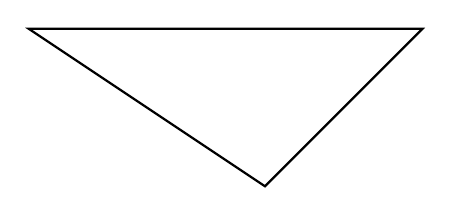
\begin{tikzpicture}
\coordinate (A) at (0,0);
\coordinate (B) at (5,0);
\coordinate (C) at (3,-2);
\draw[thick] (A)--(B)--(C)--cycle;
\end{tikzpicture}
    \end{lstlisting} & 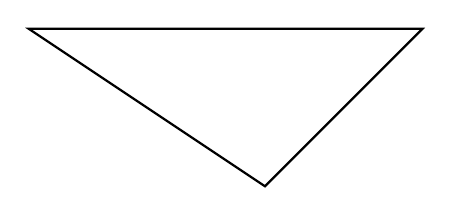
\begin{tikzpicture}
    \coordinate (A) at (0,0);
    \coordinate (B) at (5,0);
    \coordinate (C) at (3,-2);
    \draw[thick] (A)--(B)--(C)--cycle;
    \end{tikzpicture} \\
    \bottomrule
    \end{tabular}
    \caption{A triangle with tikzpicture}
    \label{tab:simpleTriangle}
\end{table}
The reason it pays to label the vertices, as in the last example, is because it make adding labels to the triangle very simple. Segments are identified by the vertices at either end, the order is important, so if the label ends up on the wrong side, just swap the order of the vertices. Angles are identified by the three vertices that make them up, with the labelled vertex in the middle. ``Why not just the middle one alone?'' you may ask. Because having the labels in one order labels the interior angle, if you reverse the order it labels the exterior angle, this is particularly useful if you are using the \lstinline|\tkzMarkAngle{}| command to put an arc on your diagram. In the latest versions of \LaTeX\ it has become the default to include a tick mark on the arc, if you don't want it, just include \lstinline|[mark=none]| before the braces.
\begin{table} [H]
    \centering
    \begin{tabular}{m{0.61\textwidth}m{0.33\textwidth}}
    \toprule
    \LaTeX\ \begin{lstinline}!\usepackage{tkz-euclide}!\end{lstinline} &  \\
    \addlinespace
    \midrule
    \begin{lstlisting}
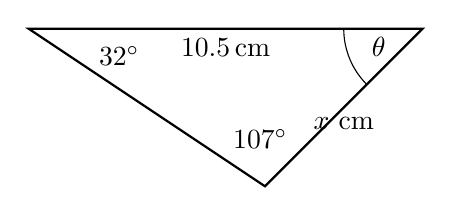
\begin{tikzpicture}
\coordinate (A) at (0,0);
\coordinate (B) at (5,0);
\coordinate (C) at (3,-2);
\draw[thick] (A)--(B)--(C)--cycle;
\tkzLabelSegment (A,B){$\SI{10.5}{\cm}$}
\tkzLabelSegment (B,C){$x$ cm}
\tkzLabelAngle[pos=1.2](C,A,B){$\ang{32}$}
\tkzLabelAngle[pos=0.6](B,C,A){$\ang{107}$}
\tkzMarkAngle[mark=none](A,B,C)
\tkzLabelAngle[pos=0.6](A,B,C){$\theta$}
\end{tikzpicture}
    \end{lstlisting} & 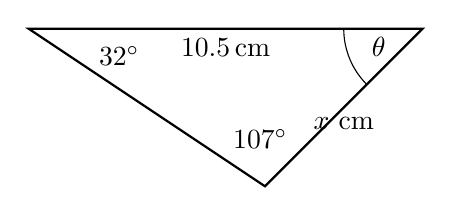
\begin{tikzpicture}
    \coordinate (A) at (0,0);
    \coordinate (B) at (5,0);
    \coordinate (C) at (3,-2);
    \draw[thick] (A)--(B)--(C)--cycle;
    \tkzLabelSegment (A,B){$\SI{10.5}{\cm}$}
    \tkzLabelSegment (B,C){$x$ cm}
    \tkzLabelAngle[pos=1.2](C,A,B){$\ang{32}$}
    \tkzLabelAngle[pos=0.6](B,C,A){$\ang{107}$}
    \tkzMarkAngle[mark=none](A,B,C)
    \tkzLabelAngle[pos=0.6](A,B,C){$\theta$}
    \end{tikzpicture} \\
    \bottomrule
    \end{tabular}
    \caption{A labelled triangle with tikzpicture and tkz-euclide}
    \label{tab:labelledTriangle}
\end{table}

\subsection{Probability}
The probability you will need to use the information in this section is quite high.
\subsubsection{Notation}
If you need to do permuations and combinations a lot, it is easy to define a couple of macros to make rendering them easier. Writing your own \LaTeX\ functions takes a little bit of effort, but you can nearly always find what you want online already.

\begin{lstlisting}
\newcommand*{\Perm}[2]{{}^{#1}\!P_{#2}}%
\newcommand*{\Comb}[2]{{}^{#1}C_{#2}}%
\end{lstlisting}

Now you have two new commands to use in the same way as other \LaTeX\ commands.

\begin{table} [H]
    \centering
    \begin{tabular}{m{0.59\textwidth}m{0.35\textwidth}}
    \toprule
    \LaTeX \\
    \addlinespace
    \midrule
    \lstinline|\Comb{6}{3}| & $\Comb{6}{3}$\\
    \addlinespace
    \midrule
    \lstinline|\Perm{n}{k}| & $\Perm{n}{k}$\\
    \bottomrule
    \end{tabular}
    \caption{Combinations and permutations}
    \label{tab:combinations}
\end{table}

\subsubsection{Dice}
Cards and dice are often used in probability questions, and it is more interesting to use a diagram than simply writing ``you roll a 6'' or ``you pick a pair of kings''. Latex offers a way of adding images, just as easily as text.

Dice are included in the \texttt{epsdice} package, it can be used to display dice graphically. As the images are small, adding the package \texttt{moresize} allows you to print them bigger.\\
\begin{table} [H]
    \centering
    \begin{tabular}{m{0.59\textwidth}m{0.35\textwidth}}
    \toprule
    \LaTeX\ \begin{lstinline}!\usepackage{epsdice}!\end{lstinline}\\
    \addlinespace
    \midrule
    \begin{lstinline} !\epsdice{5}! \end{lstinline}& \epsdice{5}\\
    \addlinespace
    \midrule
    \begin{lstinline} !\begin{HUGE} \epsdice{6} \epsdice{1} \end{HUGE}! \end{lstinline} &  \begin{HUGE} \epsdice{6} \epsdice{1} \end{HUGE}\\
    \bottomrule
    \end{tabular}
    \caption{Dice images}
    \label{tab:diceImages}
\end{table}

\subsubsection{Playing cards}
Playing cards come from \texttt{pst-poker} package, and can be used to display single cards or collections.\\
\begin{table} [H]
    \centering
    \begin{tabular}{m{0.59\textwidth}m{0.35\textwidth}}
    \toprule
    \LaTeX\ \begin{lstinline}!\usepackage{pst-poker}!\end{lstinline} & \\
    \addlinespace
    \midrule
    \begin{lstinline}!\As \fourd \Jc!\end{lstinline} & \As \fourd \Jc \\
    \addlinespace
    \midrule
    \begin{lstlisting}
\psset{backcolor=red}\crdback
\psset{backcolor=blue}\crdback
    \end{lstlisting} & \psset{backcolor=red}\crdback \psset{backcolor=blue}\crdback \\
    \addlinespace
    \midrule
    \begin{lstlisting}
\crdAs \crdfourd \crdJc
    \end{lstlisting} &
    \crdAs \crdfourd \crdJc \\
    \addlinespace
    \midrule
    \begin{lstlisting}
\newcommand\inline[1]{#1\kern-35pt 
\ignorespaces}
\inline{\crdtenh}
\inline{\crdJh}
\inline{\crdQh}
\inline{\crdKh}
\inline{\crdAh}
    \end{lstlisting} &
    \newcommand\inline[1]{#1\kern-35pt\ignorespaces}
    \inline{\crdtenh}
    \inline{\crdJh}
    \inline{\crdQh}
    \inline{\crdKh}
    \inline{\crdAh}\\
    \addlinespace
    \midrule
        \begin{lstlisting}
\newcommand\inhand[3][250pt]{
    \rotatebox[origin=b]{#2}{
    \raisebox{#1}{#3}}}
\setstackgap{L}{0pt} 
\Longunderstack{
\inhand{12}{\crdtenc}
\inhand{6}{\crdJc}
\inhand{0}{\crdQc}
\inhand{-6}{\crdKc}
\inhand{-12}{\crdAc}}
    \end{lstlisting} &
    \newcommand\inhand[3][250pt]{\rotatebox[origin=b]{#2}{\raisebox{#1}{#3}}}
    \setstackgap{L}{0pt} 
    \Longunderstack{
    \inhand{12}{\crdtenc}
    \inhand{6}{\crdJc}
    \inhand{0}{\crdQc}
    \inhand{-6}{\crdKc}
    \inhand{-12}{\crdAc}}\\
    \bottomrule
    \end{tabular}
    \caption{Playing cards}
    \label{tab:playingCards}
\end{table}



\subsubsection{Venn diagrams}

\begin{table} [H]
    \centering
    \begin{tabular}{m{0.59\textwidth}m{0.35\textwidth}}
    \toprule
    \LaTeX\ \begin{lstinline}!\usepackage{venndiagram}!\end{lstinline} & result  \\
    \addlinespace
    \midrule
	\begin{lstlisting}
\begin{venndiagram2sets}
\fillA \fillB
\end{venndiagram2sets}
	\end{lstlisting} &
    \begin{venndiagram2sets}
    \fillA \fillB
    \end{venndiagram2sets}\\
    \midrule
    \begin{lstlisting}
\begin{venndiagram2sets}
\fillACapB
\end{venndiagram2sets}
    \end{lstlisting} &
    \begin{venndiagram2sets}
    \fillACapB
    \end{venndiagram2sets} \\
    \bottomrule
    \end{tabular}
    \caption{Venn diagrams}
    \label{tab:vennDiagrams}
\end{table}

\begin{table} [H]
    \centering
    \begin{tabular}{m{\textwidth}}
    \toprule
    \LaTeX\ \begin{lstinline}!\usepackage{overpic}!\end{lstinline}\\
    \addlinespace
    \midrule
    \begin{lstlisting}
\begin{venndiagram3sets}[labelOnlyA={1},labelOnlyB={2},labelOnlyC={3},
labelOnlyAB={4},labelOnlyAC={5},labelOnlyBC={6},labelABC={7},
labelNotABC={8}]
\setpostvennhook
{
\draw[<-] (labelA) -- ++(135:3cm) node[above] {Students who eat
artichokes};
\draw[<-] (labelB) -- ++(45:3cm) node[above] {Students who eat
broccoli};
8
\draw[<-] (labelC) -- ++(-90:3cm) node[below] {Students who eat carrots};
\draw[<-] (labelABC) -- ++(0:3cm) node[right,text width=4cm,align=flush left] {7 students eat all};
\draw[<-] (labelNotABC) -- ++(-135:3cm) node[below,text width=4cm,align=flush left] {8 students don't eat any};
}
\end{venndiagram3sets}
    \end{lstlisting}\\
    \begin{center}
    \begin{venndiagram3sets}[labelOnlyA={1},labelOnlyB={2},labelOnlyC={3},
labelOnlyAB={4},labelOnlyAC={5},labelOnlyBC={6},labelABC={7},
labelNotABC={8}]
\setpostvennhook
{
\draw[<-] (labelA) -- ++(135:3cm) node[above] {Students who eat
artichokes};
\draw[<-] (labelB) -- ++(45:3cm) node[above] {Students who eat
broccoli};
8
\draw[<-] (labelC) -- ++(-90:3cm) node[below] {Students who eat carrots};
\draw[<-] (labelABC) -- ++(0:3cm) node[right,text width=4cm,align=flush left] {7 students eat all};
\draw[<-] (labelNotABC) -- ++(-135:3cm) node[below,text width=4cm,align=flush left] {8 students don't eat any};
}
\end{venndiagram3sets}
\end{center}\\
    \bottomrule
    \end{tabular}
    \caption{Annotated Venn diagram}
    \label{tab:annotatedVenn}
\end{table}
\subsection{Graphing}
Unsurprisingly, graphing is well supported in \LaTeX. From simple plots, including bar and column graphs, to more complex 3D graphs, creating anything from a plain to fully annotated graph is straightforward. The package \texttt{pgfplots} provides most of the functionality.

At its simplest, you can draw a plot with just five lines of text.

\begin{table} [H]
    \centering
    \begin{tabular}{m{0.45\textwidth}m{0.49\textwidth}}
    \toprule
    \LaTeX\ \begin{lstinline}!\usepackage{pgfplots}!\end{lstinline} &   \\
    \addlinespace
    \midrule
    \begin{lstlisting}
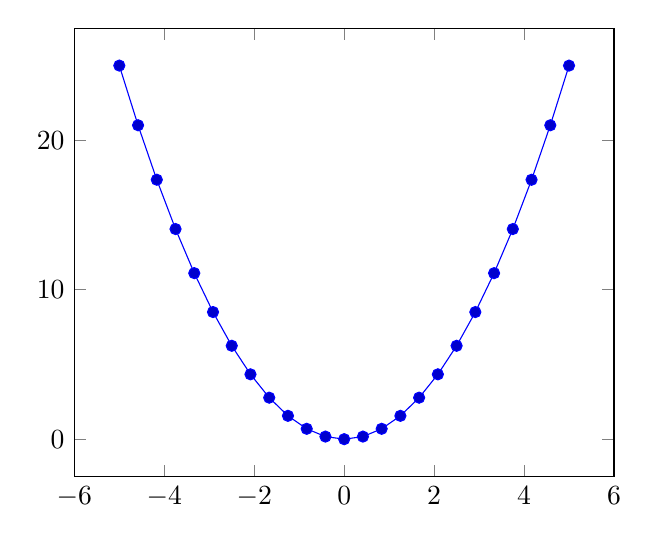
\begin{tikzpicture}
\begin{axis}
\addplot{x^2};
\end{axis}
\end{tikzpicture}[width=60mm]
    \end{lstlisting} &
    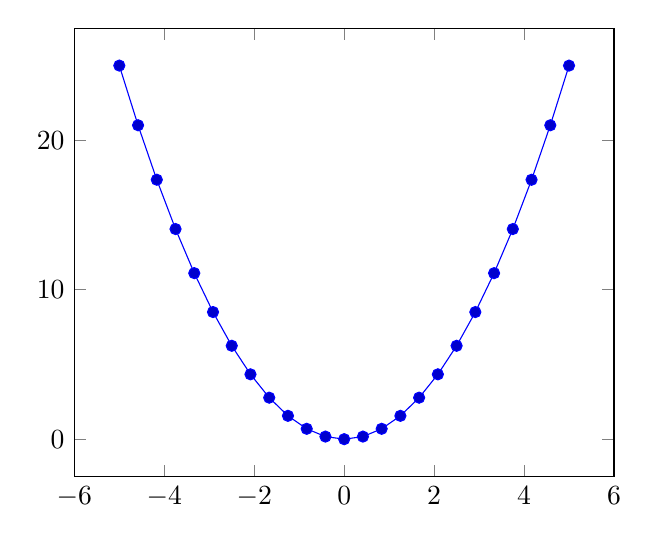
\begin{tikzpicture}
    \begin{axis}
        \addplot{x^2};
    \end{axis}
\end{tikzpicture} \\
    \bottomrule
    \end{tabular}
    \caption{A simple 2D plot with pgfplots}
    \label{tab:simple2Dplot}
\end{table}

\begin{table} [H]
    \centering
    \begin{tabular}{m{0.49\textwidth}m{0.45\textwidth}}
    \toprule
    \LaTeX\ \begin{lstinline}!\usepackage{pgfplots}!\end{lstinline} &   \\
    \addlinespace
    \midrule
	\begin{lstlisting}
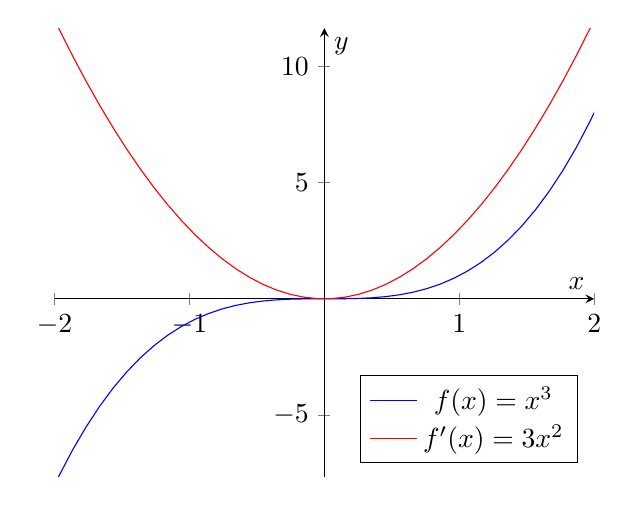
\begin{tikzpicture}
\begin{axis}[xmin=-2, xmax=2,
axis lines=middle,
xlabel=$x$,
ylabel=$y$,
legend pos=south east]
\addplot[color=blue,samples=100]{x^3};
\addplot[color=red,samples=100]{3*x^2};
\addlegendentry{$f(x)=x^3$}
\addlegendentry{$f'(x)=3x^2$}
\end{axis}
\end{tikzpicture}
	\end{lstlisting} &
     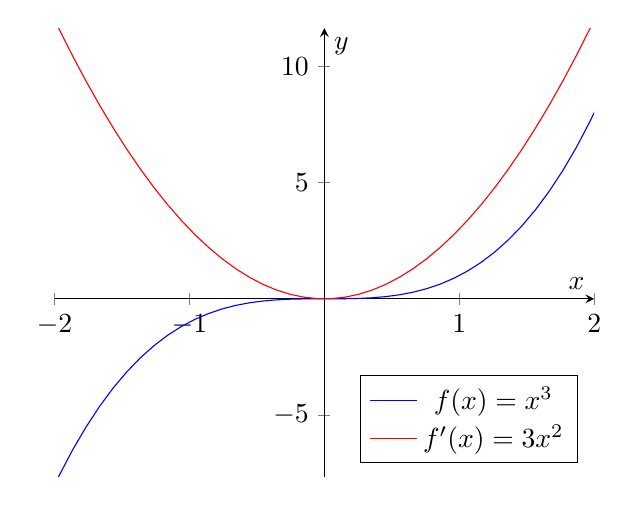
\begin{tikzpicture}
    \begin{axis}[xmin=-2, xmax=2,
    axis lines=middle,
    xlabel=$x$,
    ylabel=$y$,
    legend pos=south east]
        \addplot[color=blue, samples=100]{x^3};
        \addplot[color=red, samples=100]{3*x^2};
    \addlegendentry{$f(x)=x^3$}
    \addlegendentry{$f'(x)=3x^2$}
    \end{axis}
\end{tikzpicture}\\
    \bottomrule
    \end{tabular}
    \caption{Function graphs}
    \label{tab:functionGraphs}
\end{table}

\begin{table} [H]
    \centering
    \begin{tabular}{m{0.49\textwidth}m{0.45\textwidth}}
    \toprule
    \LaTeX\ \begin{lstinline}!\usepackage{pgfplots}!\end{lstinline} &  \\
    \addlinespace
    \midrule
	\begin{lstlisting}
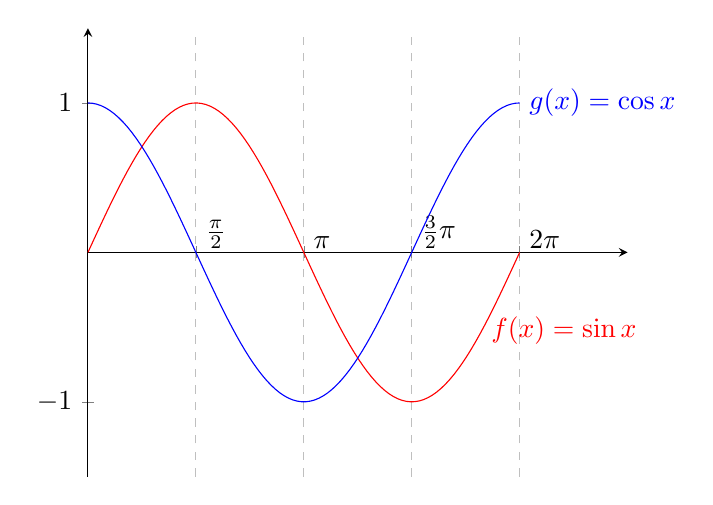
\begin{tikzpicture}
\begin{axis}[clip=false,
xmin=0,xmax=2.5*pi,
ymin=-1.5,ymax=1.5,
axis lines=middle,
xtick={0,pi/2,pi,3*pi/2,2*pi},
xticklabels={$0$,$\frac{\pi}{2}$,$\pi$,$\frac{3}{2}\pi$,$2\pi$},
xticklabel style={anchor=south west},
xmajorgrids=true,
grid style=dashed
]
\addplot[domain=0:2*pi,red, samples=100]{sin(deg(x))}
node[right, pos=0.9]{$f(x)=\sin x$};
\addplot[domain=0:2*pi,blue, samples=100]{cos(deg(x))}
node[right, pos=1.0]{$g(x)=\cos x$};
\end{axis}
\end{tikzpicture}
	\end{lstlisting} &
 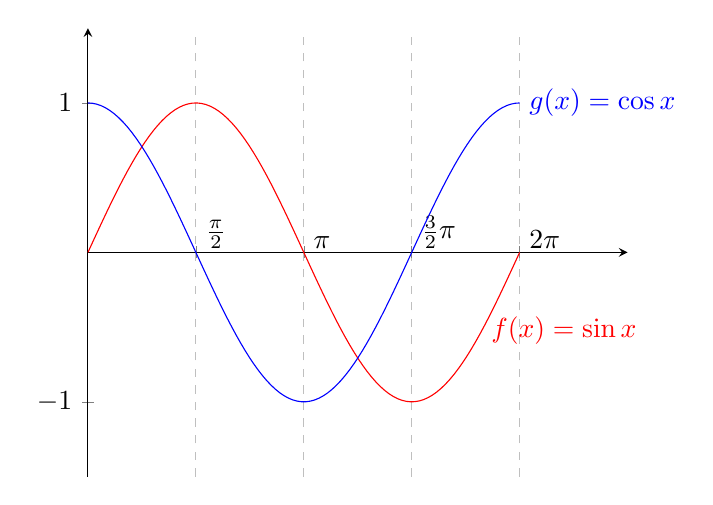
\begin{tikzpicture}
    \begin{axis}[clip=false,
    xmin=0,xmax=2.5*pi,
    ymin=-1.5,ymax=1.5,
    axis lines=middle,
    xtick={0,pi/2,pi,3*pi/2,2*pi},
    xticklabels={$0$,$\frac{\pi}{2}$,$\pi$,$\frac{3}{2}\pi$,$2\pi$},
    xticklabel style={anchor=south west},
    xmajorgrids=true,
    grid style=dashed
    ]
    \addplot[domain=0:2*pi,red, samples=100]{sin(deg(x))}
    node[right, pos=0.9]{$f(x)=\sin x$};
    \addplot[domain=0:2*pi,blue, samples=100]{cos(deg(x))}
    node[right, pos=1.0]{$g(x)=\cos x$};
    \end{axis}
\end{tikzpicture}\\
    \bottomrule
    \end{tabular}
    \caption{Trigonometric plots}
    \label{tab:trigonometricPlots}
\end{table}

\begin{table} [H]
    \centering
    \begin{tabular}{m{0.49\textwidth}m{0.45\textwidth}}
    \toprule
    \LaTeX\ \begin{lstinline}!\usepackage{pgfplots}!\end{lstinline} &  \\
    \addlinespace
    \midrule
	\begin{lstlisting}
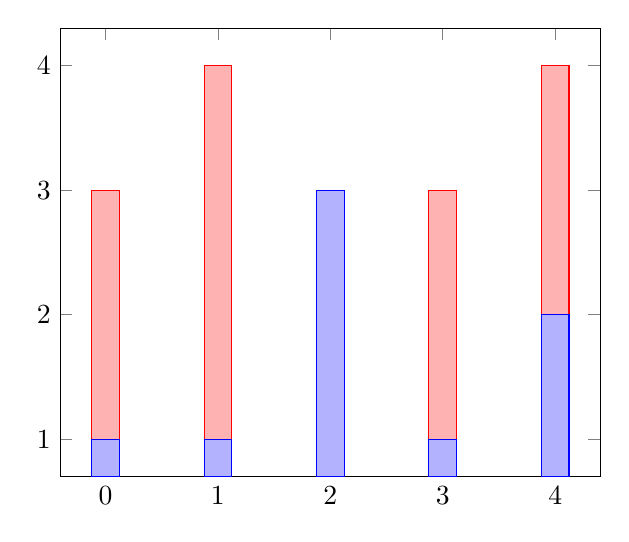
\begin{tikzpicture}
\begin{axis}[ybar stacked]
\addplot coordinates {(0,1) (1,1) (2,3) (3,1) (4,2)};
\addplot coordinates {(0,2) (1,3) (2,0) (3,2) (4,2)};
\end{axis}
\end{tikzpicture}
\end{lstlisting} &
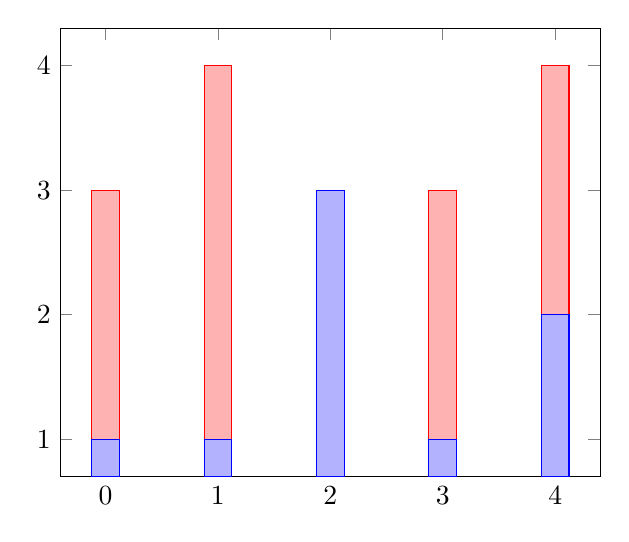
\begin{tikzpicture}
    \begin{axis}[ybar stacked]
    \addplot coordinates {(0,1) (1,1) (2,3) (3,1) (4,2)};
    \addplot coordinates {(0,2) (1,3) (2,0) (3,2) (4,2)};
    \end{axis}
\end{tikzpicture}\\
    \bottomrule
    \end{tabular}
    \caption{Stacked bar graph}
    \label{tab:stackedBar}
\end{table}

\begin{table} [H]
    \centering
    \begin{tabular}{m{0.49\textwidth}m{0.45\textwidth}}
    \toprule
    \LaTeX\ \begin{lstinline}!\usepackage{pgfplots}!\end{lstinline} &  \\
    \addlinespace
    \midrule
	\begin{lstlisting}
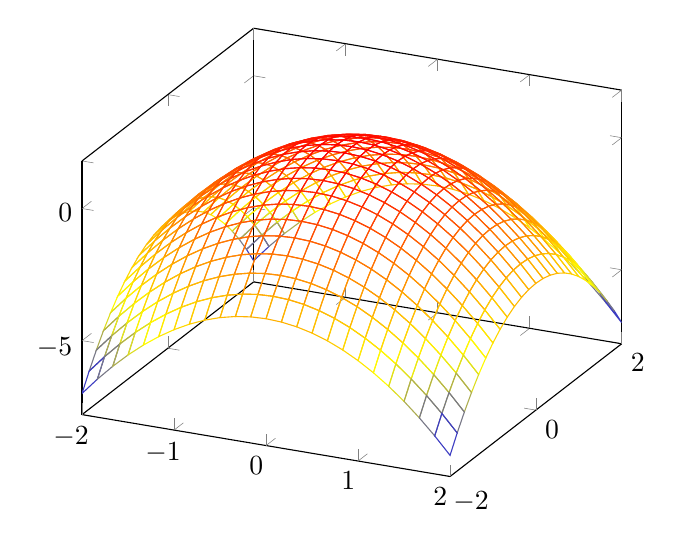
\begin{tikzpicture}
    \begin{axis}[colormap/hot]
        \addplot3[mesh, samples=25, domain=-2:2]{1-x^2-y^2};
    \end{axis}
\end{tikzpicture}
\end{lstlisting} &
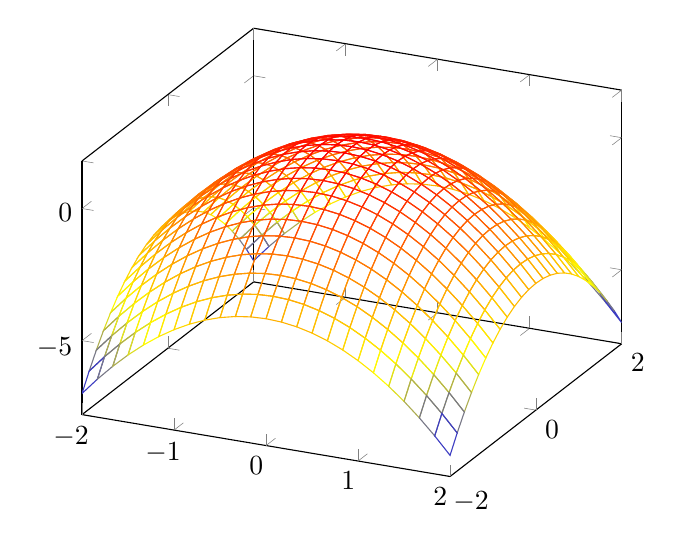
\begin{tikzpicture}
    \begin{axis}[colormap/hot]
        \addplot3[mesh, samples=25, domain=-2:2]{1-x^2-y^2};
    \end{axis}
\end{tikzpicture}\\
    \bottomrule
    \end{tabular}
    \caption{3D graph}
    \label{tab:3dGraph}
\end{table}
\section{\LaTeX\ for Physics}
A lot of Physics is just Maths, so all the support we have seen for setting mathematical text is every bit as useful in Physics. One particularly useful addition for Physics (and most other technical fields) is the support for SI measurements. Adding the package \texttt{siunitx} will allow quantities, including units, to be easily displayed in a document, formatted in the standard manner.

\begin{table} [H]
    \centering
    \begin{tabular}{m{0.59\textwidth}m{0.35\textwidth}}
    \toprule
    \LaTeX\ \begin{lstinline}!\usepackage{siunitx}!\end{lstinline} &  \\
    \addlinespace
    \midrule
    \begin{lstinline}!\SI{2}{\metre\per\second}!\end{lstinline} &
        \SI{2}{\metre\per\second} \\
    \addlinespace
    \midrule
    \begin{lstinline}!\SI{42.9}{\kilogram}!\end{lstinline} &
        \SI{42.9}{\kilogram} \\
    \addlinespace
    \midrule
    \begin{lstinline}!\SI{3.8}{\newton} or \SI{3.8}{\kilogram\metre\per\second\squared}!\end{lstinline} &
        \SI{3.8}{\newton} or \SI{3.8}{\kilogram\metre\per\second\squared} \\	
    \bottomrule
    \end{tabular}
    \caption{Metric measurements}
    \label{tab:metricMeasurements}
\end{table}

Notice that you can use \texttt{\textbackslash metre} for metres; you don't have to use the US spelling; unfortunately, colour is still \texttt{\textbackslash color}.
\subsection{Vector diagrams}
Vectors are just arrows, and \LaTeX has no trouble working with them. It's just a variation on the drawing we saw for triangles. Often though, we want a more interesting diagram; maybe we want the vectors to be overlaid on an image of some billiard balls or on an aircraft. \LaTeX can do this, but it can be a bit fiddly getting everything lined up.

Although you can adjust the opacity of elements within \LaTeX\ I simply used a version of the light plane graphic adjusted to a 50\% opacity rather than changing it in \LaTeX.\\
\vspace{5mm}
\begin{center}
\begin{overpic}[abs,unit=1mm,scale=0.50]{LightPlane50.png}
    \put(-20,-10){
    \begin{tikzpicture}
        \coordinate (A) at (5,5);
        \coordinate (B) at (5,7);
        \coordinate (C) at (5,3);
        \coordinate (D) at (2,5);
        \coordinate (E) at (8,5);
        \draw[thick, -latex] (A)--(B) node[anchor=north west] {lift};
        \draw[thick, -latex] (A)--(C) node[anchor=south west] {weight};
        \draw[thick, -latex] (A)--(D) node[anchor=east] {thrust};
        \draw[thick, -latex] (A)--(E) node[anchor=west] {drag};
    \end{tikzpicture}}
\end{overpic}
\end{center}
\vspace{8mm}
Ok, there's a trick to getting things aligned. If you want to overlay one diagram on the other, you can make it much easier on yourself by doing it in two steps. You start by adding in the image and overlaying it with a grid.

\begin{table} [H]
    \centering
    \begin{tabular}{m{0.46\textwidth}m{0.48\textwidth}}
    \toprule
    \LaTeX\ \begin{lstinline}!\usepackage{overpic}!\end{lstinline} &  \\
    \addlinespace
    \midrule
	\begin{lstlisting}
\begin{overpic}[abs,unit=1mm,scale=0.50,grid]{LightPlane50.png}
\end{overpic}    
	\end{lstlisting} & 
 \begin{overpic}[abs,unit=1mm,scale=0.50,grid]{LightPlane50.png}
\end{overpic}\\
    \bottomrule
    \end{tabular}
    \caption{Vector overlay - Step 1}
    \label{tab:vectorOverlay1}
\end{table}

Then, using the grid you can work out the position for the \texttt{\textbackslash put} command. You need to remember a couple of things. The \texttt{\textbackslash tikzpicture} has its origin in the lower left corner, so you are placing things relative to that point. Also the units in \texttt{\textbackslash tikzpicture} are in centimetres; our grid is in millimetres, so the offset will be 10x the \texttt{\textbackslash tikzpicture} units. Don't forget to remove the \texttt{grid} option from the \texttt{\textbackslash begin\{overpic\}} command.

\begin{table} [H]
    \centering
    \begin{tabular}{m{\textwidth}}
    \toprule
    \LaTeX\ \begin{lstinline}!\usepackage{overpic}!\end{lstinline}\\
    \addlinespace
    \midrule
    \begin{lstlisting}
\begin{overpic}[abs,unit=1mm,scale=0.50]{LightPlane50.png}
\put(-20,-10){
\begin{tikzpicture}
\coordinate (A) at (5,5);
\coordinate (B) at (5,7);
\coordinate (C) at (5,3);
\coordinate (D) at (2,5);
\coordinate (E) at (8,5);
\draw[thick, -latex] (A)--(B) node[anchor=north west] {lift};
\draw[thick, -latex] (A)--(C) node[anchor=south west] {weight};
\draw[thick, -latex] (A)--(D) node[anchor=east] {thrust};
\draw[thick, -latex] (A)--(E) node[anchor=west] {drag};
\end{tikzpicture}}
\end{overpic}
    \end{lstlisting}\\
    \begin{center}
    \begin{overpic}[abs,unit=1mm,scale=0.50]{LightPlane50.png}
    \put(-20,-10){
    \begin{tikzpicture}
        \coordinate (A) at (5,5);
        \coordinate (B) at (5,7);
        \coordinate (C) at (5,3);
        \coordinate (D) at (2,5);
        \coordinate (E) at (8,5);
        \draw[thick, -latex] (A)--(B) node[anchor=north west] {lift};
        \draw[thick, -latex] (A)--(C) node[anchor=south west] {weight};
        \draw[thick, -latex] (A)--(D) node[anchor=east] {thrust};
        \draw[thick, -latex] (A)--(E) node[anchor=west] {drag};
    \end{tikzpicture}}
\end{overpic}
\end{center}\\
    \bottomrule
    \end{tabular}
    \caption{Vector overlay - Step 2}
    \label{tab:vectorOverlay2}
\end{table}
\subsection{Nuclear physics, etc}
The best package for setting out nuclear physics equations is the package designed for chemistry, \textbf{mhchem}. The four corners of a symbol can each hold a piece of information, the package lets you arrange them easily using the \lstinline|\ce| command. To access the corners on the left, place the annotations before the symbol, to access the corners on the right, place the annotations after the symbol. In both cases, the top corner is selected by putting a caret before the value, the lower corner is chosen by putting an underscore before the value. Also, because it's from a chemistry package \lstinline|\ce| also turns \lstinline|->| into $\ce{->}$.

\lstinline|\ce{^1_2Z^3_4}| becomes $\ce{^1_2Z^3_4}$
\begin{table} [H]
    \centering
    \begin{tabular}{m{0.55\textwidth}m{0.39\textwidth}}
    \toprule
    \LaTeX\ \begin{lstinline}!\usepackage{mhchem}!\end{lstinline} &  \\
    \addlinespace
    \midrule
    \lstinline|$\ce{^1_1H + ^1_1H -> ^2_1H + e^+ + $\nu$_e}$| & $\ce{^1_1H + ^1_1H -> ^2_1H + e^+ + $\nu$_e}$\\    
    \begin{lstinline}!$\ce{e^+ + e^- -> $\gamma$ + \SI{1.442}{\mega\eV}}$!\end{lstinline} & $\ce{e^+ + e^- -> $\gamma$ + \SI{1.442}{\mega\eV}}$\\
    \begin{lstinline}!$\ce{^2_1H + ^1_1H -> ^3_2He + $\gamma$ + \SI{5.493}{\mega\eV}}$!\end{lstinline} & $\ce{^2_1H + ^1_1H -> ^3_2He + $\gamma$ + \SI{5.493}{\mega\eV}}$\\
    \bottomrule
    \end{tabular}
    \caption{Nuclear reactions}
    \label{tab:nuclearReactions}
\end{table}
Notice that in the expressions that contain Greek letters, you have to surround the code for the Greek letter with \lstinline|$ $|; otherwise, it won't print. This is caused by an interaction between the \textbf{mhchem} package and the standard mathematics font. If you find other characters disappearing, this trick will probably bring them back too.

Along the lines of, ``you can find almost anything in \LaTeX'' is a command that will print out a representation of an atomic nucleus.
\begin{table} [H]
    \centering
    \begin{tabular}{m{0.74\textwidth}m{0.20\textwidth}}
    \toprule
    \LaTeX\ \begin{lstinline}!\usetikzlibrary{calc}!\end{lstinline} &  \\
    \addlinespace
    \midrule
	\begin{lstlisting}

\begin{tikzpicture}
\path (-2,-2) rectangle (2,2);
\pgfmathdeclarerandomlist{color}{{red}{white}}
\pgfmathsetseed{1}
\foreach \A/\R in {25/1,12/0.9,15/0.8,20/0.7,12/0.5,7/0.3,1/0}
{\pgfmathsetmacro{\S}{360/\A}
\foreach \B in {0,\S,...,360}{
\pgfmathrandomitem{\C}{color}
\shade[ball color=\C] (\B+\A:\R) circle (5pt);}}
\node at (-1,1.3) {\ce{^{226}_{88}Ra}};
\end{tikzpicture}	    
	\end{lstlisting} &

\begin{tikzpicture}
\path (-2,-2) rectangle (2,2);
\pgfmathdeclarerandomlist{color}{{red}{white}}
\pgfmathsetseed{1}
\foreach \A/\R in {25/1,12/0.9,15/0.8,20/0.7,12/0.5,7/0.3,1/0}{
      \pgfmathsetmacro{\S}{360/\A}
           \foreach \B in {0,\S,...,360}{
               \pgfmathrandomitem{\C}{color}
               \shade[ball color=\C] (\B+\A:\R) circle (5pt);
           }
}
\node at (-1,1.3) {\ce{^{226}_{88}Ra}};
\end{tikzpicture}    \\
    \bottomrule
    \end{tabular}
    \caption{Nucleus picture}
    \label{tab:nucleusPicture}
\end{table}

\subsection{Circuit Diagrams}
The built-in drawing package in \LaTeX\ has been extended by many users, making it very simple to add specialised diagrams. A good example from the Science syllabus is adding a circuit diagram. If you are going to get really complex, there are better packages available, but for high school work, it's fine.

The code is very similar to other drawing functions, but you substitute the circuit elements where you would normally put lines in your diagram.

\begin{table} [H]
    \centering
    \begin{tabular}{m{\textwidth}}
    \toprule
    \LaTeX\ \begin{lstinline}!\usepackage{circuitikz}!\end{lstinline}\\
    \addlinespace
    \midrule
    \begin{lstlisting}
\begin{circuitikz}
\draw (0,0) to[battery, l=$\SI{6.0}{\volt}$] (0,3)
to[ammeter] (5,3) -- (5,0)
to[resistor, l=$\SI{15}{\ohm}$] (0,0);
\draw (1,0) -- (1.0,-1.5)
to[voltmeter] (4.0,-1.5) -- (4.0,0);
\end{circuitikz}
    \end{lstlisting}\\
    \begin{center}
        \begin{circuitikz}
    	\draw (0,0) to[battery, l=$\SI{6.0}{\volt}$] (0,3)
    	    to[ammeter] (5,3) -- (5,0)
    	    to[resistor, l=$\SI{15}{\ohm}$] (0,0);
	    \draw (1,0) -- (1.0,-1.5)
	        to[voltmeter] (4.0,-1.5) -- (4.0,0);
	    \end{circuitikz}
     \end{center}\\
    \bottomrule
    \end{tabular}
    \caption{Circuit diagram}
    \label{tab:circuitDiagram}
\end{table}	
\section{\LaTeX\ and Chemistry}
\subsection{Chemical equations}
We've already seen the \textbf{mhchem} package earlier. The \lstinline|\ce| command allows you to place annotations around larger text, making it perfect for chemical equations, including ionic information too.
\begin{table} [H]
    \centering
    \begin{tabular}{m{0.40\textwidth}m{0.54\textwidth}}
    \toprule
    \LaTeX\ \begin{lstinline}!\usepackage{mhchem}!\end{lstinline} &  \\
    \addlinespace
    \midrule
	\begin{lstinline}!$\ce{2KI_{(aq)} + Pb(NO_3)_{2(aq)} -> 2KNO_{3(aq)} + PbI_{2(s)}}$!\end{lstinline} & $\ce{2KI_{(aq)} + Pb(NO_3)_{2(aq)} -> 2KNO_{3(aq)} + PbI_{2(s)}}$\\
    \addlinespace
    \midrule
	\begin{lstinline}!$\ce{2I^+ + Pb^{2+} -> PbI_2}$!\end{lstinline} & $\ce{2I^+ + Pb^{2+} -> PbI_2}$\\
    \bottomrule
    \end{tabular}
    \caption{Chemical reactions}
    \label{tab:chemicalReactions}
\end{table}
\subsection{Chemistry diagrams}
\subsubsection{Lewis structures}
The \textbf{lewis} package lets you put dots around a symbol representing the electrons in the outer shell.
\begin{table} [H]
    \centering
    \begin{tabular}{m{0.59\textwidth}m{0.35\textwidth}}
    \toprule
    \LaTeX\ \begin{lstinline}!\usepackage{lewis}!\end{lstinline} & result  \\
    \addlinespace
    \midrule
	\begin{lstlisting}
\lewis{O}{.}{.}{.}{}{}{}{}{.}
\hspace{-0.5em}=\,C\,
=\hspace{-0.75em}
\lewis{O}{}{}{}{.}{.}{.}{.}{}
	\end{lstlisting} &
 \lewis{O}{.}{.}{.}{}{}{}{}{.}\hspace{-0.5em}=\,
C\,
=\hspace{-0.75em}\lewis{O}{}{}{}{.}{.}{.}{.}{}\\
    \bottomrule
    \end{tabular}
    \caption{Lewis structures}
    \label{tab:lewisStructures}
\end{table}
\subsubsection{Molecular diagrams}
There are a number of packages that have been designed to draw out molecular diagrams. One of the more popular recent packages is \textbf{chemfig} it can draw quite sophisticated diagrams well beyond the needs of high school chemistry. Using it is beyond the scope of this document, but there is a wealth of information, and a complete set of documentation available online. Here's an example.
\begin{table} [H]
    \centering
    \begin{tabular}{m{\textwidth}}
    \toprule
    \LaTeX\ \begin{lstinline}!\usepackage{chemfig}!\end{lstinline}\\
    \addlinespace
    \midrule
    \begin{lstlisting}
\chemfig{CH_3CH_2-[:-60,,3]C(-[:-120]H_3C)=C(-[:-60]H)-[:60]C{(}CH_3{)}_3}
    \end{lstlisting}\\
    \begin{center}
        \chemfig{CH_3CH_2-[:-60,,3]C(-[:-120]H_3C)=C(-[:-60]H)-[:60]C{(}CH_3{)}_3}
     \end{center}\\
    \bottomrule
    \end{tabular}
    \caption{Molecular structure diagram}
    \label{tab:molecularStructure}
\end{table}	
\subsubsection{The Bohr model}
The Bohr model of the atom is important in both Chemistry and Physics. The \textbf{bohr} package provides two ways of drawing the electron shells, the simplified method used in Stage 5 Chemistry and the more accurate quantum model used in higher level courses.

In the first example the \textbf{elements} package has been used to add the electron configuration. That package contains many different pieces of information that can be added just by referencing the element name or its symbol. Although all that information is obtainable online, using the package means that if you reuse a question, you can just change the selected element and the other data will update.
\begin{table} [H]
    \centering
    \begin{tabular}{m{0.69\textwidth}m{0.25\textwidth}}
    \toprule
    \LaTeX\ \begin{lstinline}!\usepackage{bohr, elements}!\end{lstinline} &  \\
    \addlinespace
    \midrule
	\begin{lstlisting}
\setbohr{distribution-method=quantum,insert-missing}
\elconf{Fe} \\
\bohr{}{Fe}
    \end{lstlisting} &
\setbohr{distribution-method=quantum,insert-missing}
\elconf{Fe}
\bohr{}{Fe}\\
    \addlinespace
    \midrule
	\begin{lstlisting}
\setbohr{distribution-method=periodic,insert-missing}
\bohr{}{Fe}
    \end{lstlisting} &
\setbohr{distribution-method=periodic,insert-missing}
\bohr{}{Fe}
    \\
    \bottomrule
    \end{tabular}
    \caption{Bohr atoms}
    \label{tab:bohrAtoms}
\end{table}
\section{Exam papers and worksheets}
Because \LaTeX\ came out of the university environment, it's not surprising that it is pretty good at handling exams. It offers so much convenience and flexibility that it is one of the best reasons for moving to \LaTeX\ for exam setting.

\LaTeX\ comes with an exam template, you can access it by using \begin{lstinline}!\documentclass[a4paper, addpoints, 12pt]{exam}!\end{lstinline} as the first line in your document. The \texttt{addpoints} option is needed if you're going to take advantage of the additional marking tools the exam template provides. \texttt{12pt} sets the base text size for the document.
\subsection{Questions and marks}
In addition to just setting out the questions nicely, the exam package also lets questions be allocated marks, and then those marks are summed, manipulated and added to the printed pages. As we'll see in the next section, modifications that change the marking scheme are also handled automatically.

When you are in an exam document, each question starts with the \texttt{\textbackslash question[]} command. Inside the brackets, you put the number of marks for the question. More about marks a little later.

\begin{table} [H]
    \centering
    \begin{tabular}{m{0.47\textwidth}m{0.47\textwidth}}
    \toprule
    \LaTeX\ \begin{lstinline}!\documentclass{exam}!\end{lstinline} &  \\
    \addlinespace
    \midrule
	\begin{lstinline}!\question[1] A cricket ball is thrown vertically upwards. Which of the following statements about its motion is NOT true after the ball leaves the thrower's hand?!\end{lstinline} & \textbf{4.} A cricket ball is thrown vertically upwards. Which of the following statements about its motion is NOT true after the ball leaves the thrower's hand?\\
    \bottomrule
    \end{tabular}
    \caption{A multiple choice question - answers not shown}
    \label{tab:question}
\end{table}
In this case, the question is worth 1 mark; that's in the brackets. In the printed version, the number 4 is shown; that's the number of the question in sequence. \LaTeX\ keeps track of all the questions in the exam and numbers them sequentially; if you change the order of the questions, it will renumber them automatically.

\LaTeX\ does not show the marks for a question automatically, but it will if we tell it to. Not only will it show the marks for each question, but it can also show the total marks for the page and the total marks for the whole exam. This is not bad, but as we'll see when we look at creating modified exams, it will adjust the totals to take into account any modifications we make.
\begin{table} [H]
    \centering
    \begin{tabular}{m{\textwidth}}
    \toprule
    \LaTeX\ \begin{lstinline}!\usepackage{amsmath}!\end{lstinline}\\
    \addlinespace
    \midrule
	\begin{lstlisting}
\question[5] A police car is stationary at a set of traffic lights that are showing red. A person in a Bugatti drives through the lights with a speed of $\SI{72}{\kilo\metre\per\hour}$. They are too self-involved to notice the police car and continue onward without accelerating or braking. It takes the police officer $\SI{1}{\second}$ to react, they then accelerate at a constant rate of $\SI{4}{\metre\per\second\squared}$.\\
\begin{parts}
\part How much time does it take for the police officer to catch up to the Bugatti?
\vspace{50mm}
\part Over what distance does the chase take place?
\end{parts}
\ansl{50mm}	    
	\end{lstlisting}\\
    \begin{center}
    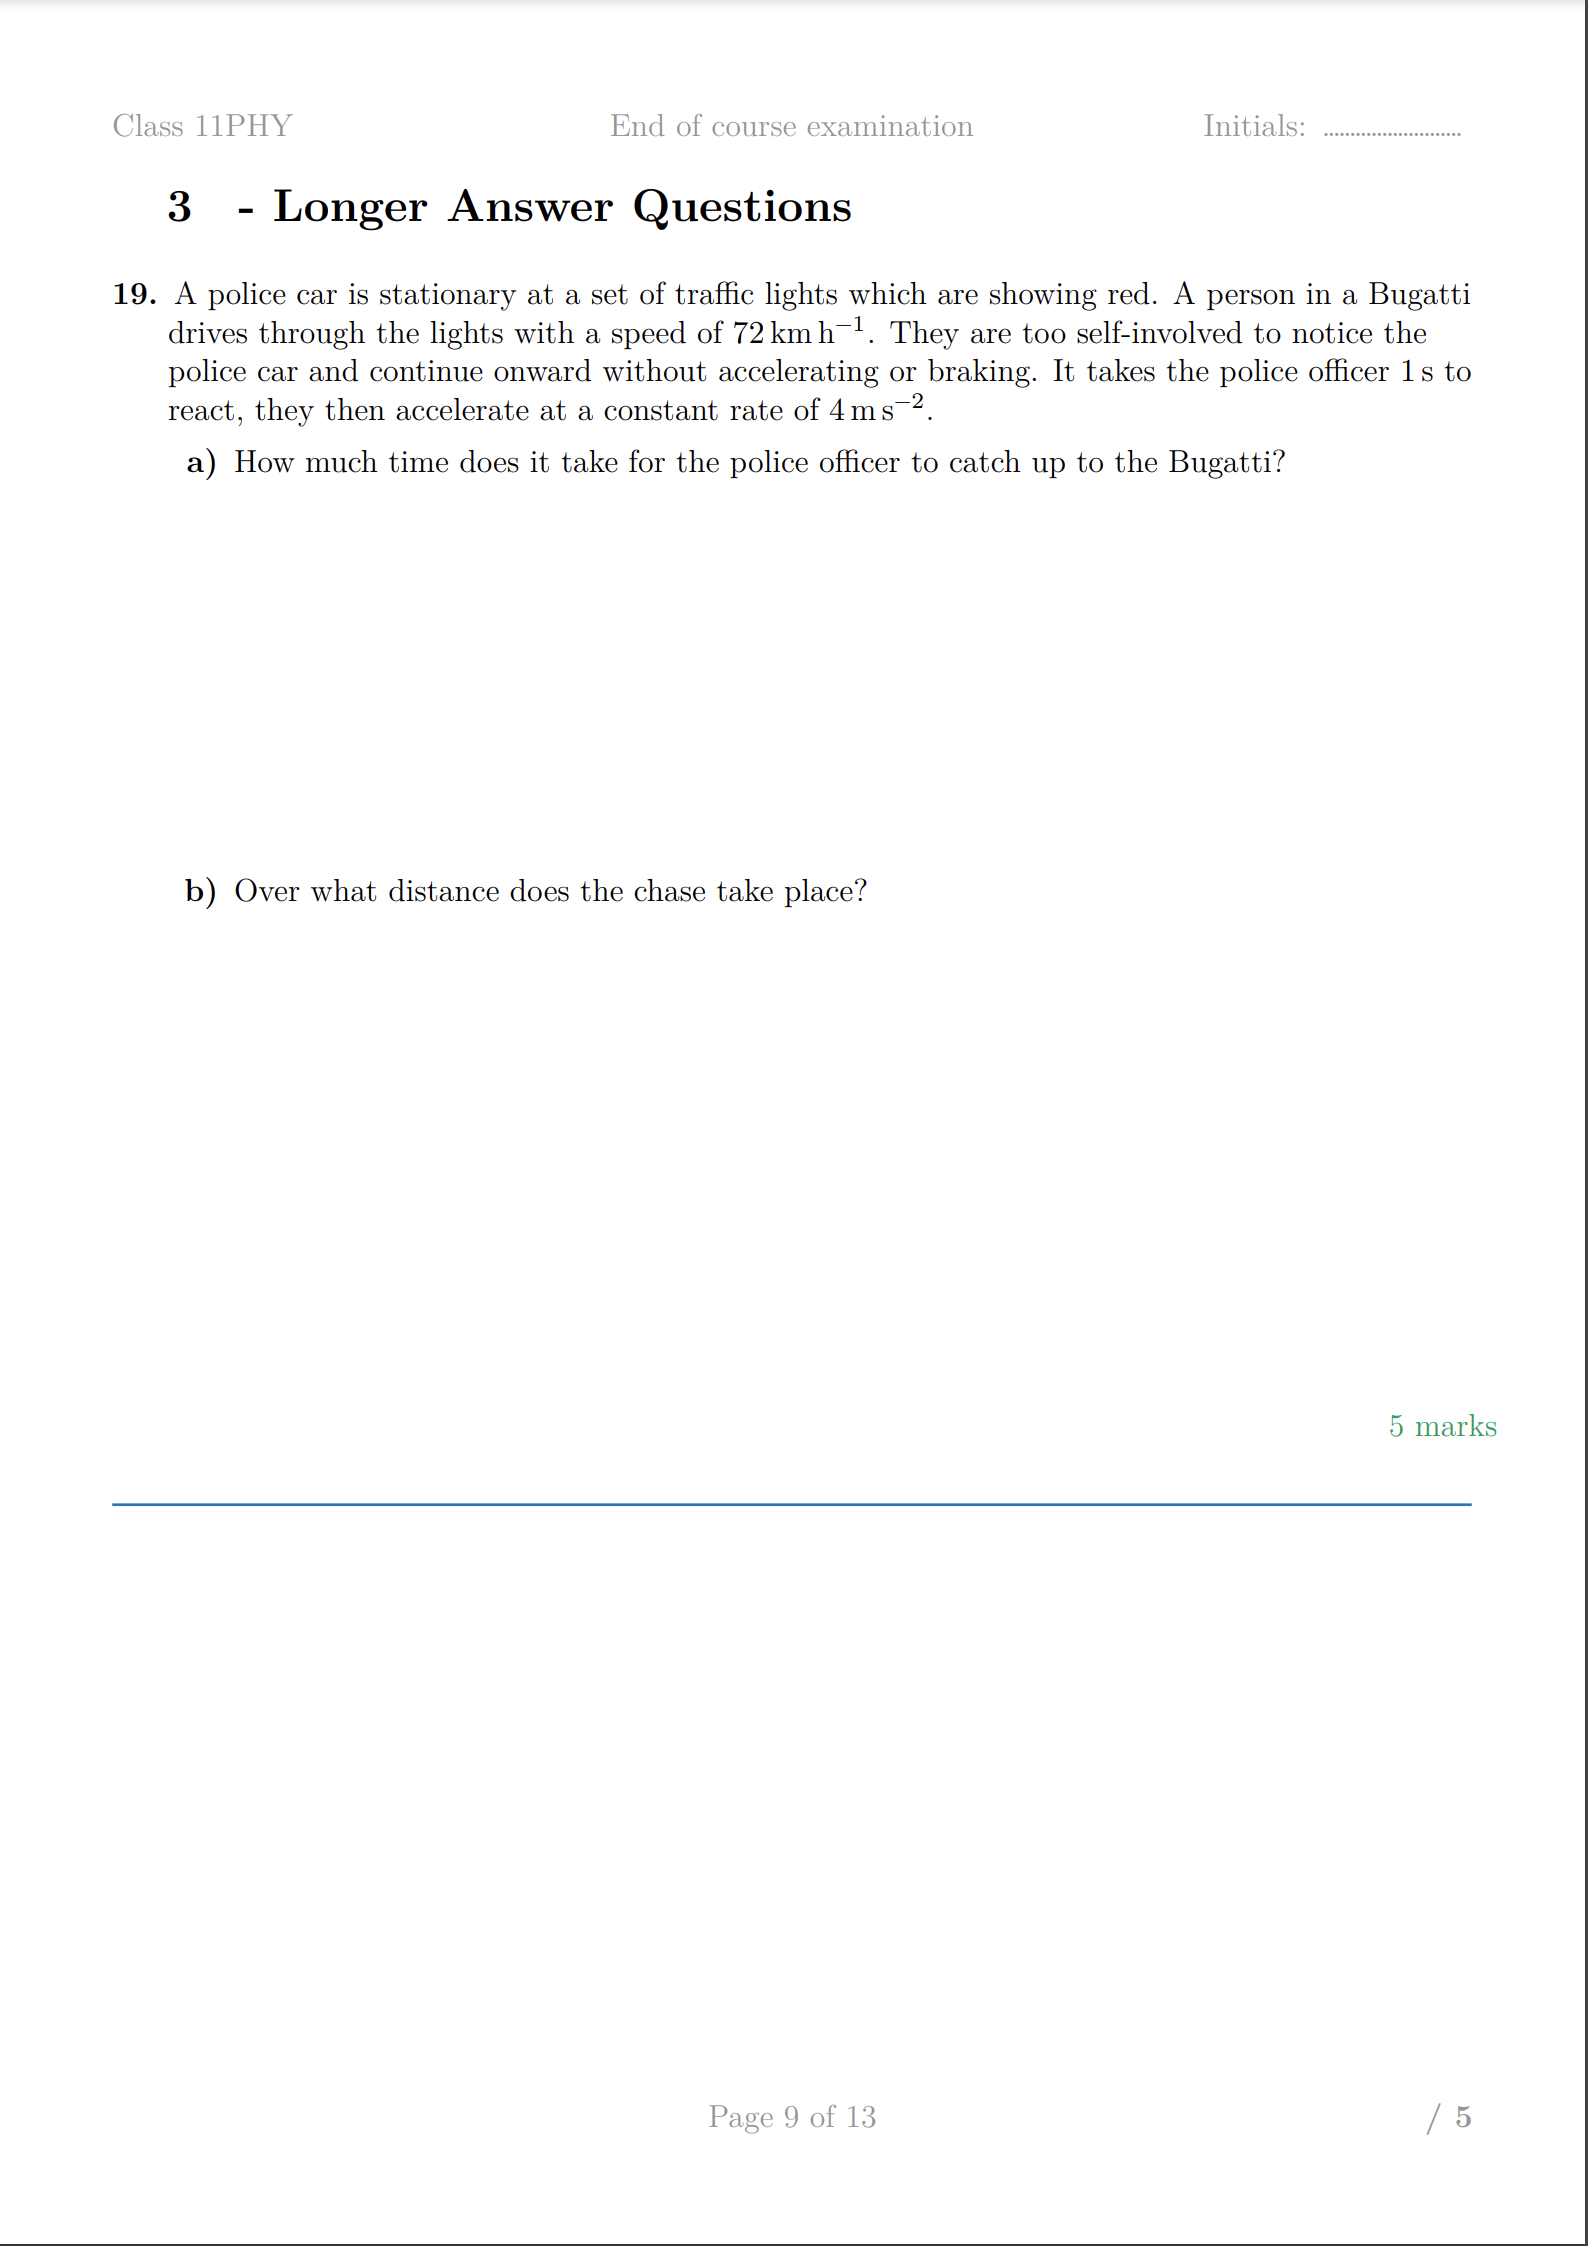
\includegraphics[scale=0.30]{Screenshot long question.png}
    \end{center}\\
    \bottomrule
    \end{tabular}
    \caption{Long answer question with marks}
    \label{tab:longAnswer}
\end{table}

There are many ways of setting out an exam page. For example, I prefer not to put lines for working; this allows a student's innate freedom to flow in how they arrange their work; the real reason is that they never use them and just write anywhere anyway. I like a line between the questions for easier marking, and I want the marks easily visible so that a student can plan their time. \LaTeX\ lets me do this with a single command \begin{lstinline}!\ansl{50mm}!\end{lstinline}. This isn't a built-in command; I made it up and include it in the preamble of all my exams.

Here's how.
\label{anslCode}
\begin{itemize}
\item Firstly, we set up a command for displaying marks without a line:
\begin{lstlisting}
\newcommand{\ans}[1]{
    \vspace{#1}
    \begin{flushright}
        \hspace{1pt} %needed to put marks at the bottom
    \end{flushright}
    \droppoints}
\end{lstlisting}
Notice the \textbf{[1]} in the first line; this tells \LaTeX that we are going to supply one piece of data when we use the command; in this case, I add the measurement that specifies how much blank space to leave.
\item Then, we use the first command in a second command that adds the line:
\begin{lstlisting}
\newcommand{\ansl}[1]{
    \ans{#1}
    \fullwidth{\noindent \color{RoyalBlue} \rule{\textwidth}{1pt}}}
\end{lstlisting}
We use the first command we defined here, just adding the full-width line.
\item Lastly, we tell \LaTeX\ how we want the marks formatted for printing. We do this in the body of the document before we write any of the questions:
\begin{lstlisting}
\begin{questions}
    \pointsdroppedatright
    \marksnotpoints
    \marginpointname{ \points}
    \setlength{\rightpointsmargin}{20mm}
    \pointformat{\color{ForestGreen} \themarginpoints\hspace{2mm}}
\end{lstlisting}
\end{itemize}
To be honest, it took a bit of trial and error to get this right, but now it exists; I just use it in all my exams. It's really simple.
\subsection{Multiple choice}
Multiple choice questions are popular in many exams, so it's not surprising that \LaTeX\ has good support for them. \LaTeX\ offers a number of automated options:
\begin{itemize}
    \item List the answers with generated letters A, B, etc
    \item Have bubbles that students can colour in on the paper.
\end{itemize}
I have switched to having colour-in bubbles on the exam paper, which means students make fewer transposition errors when answering, and it means that everything stays together in one document for marking, recording and returning. Not having multiple choice answer sheets getting separated from the rest of the exam is great.

Doing a multiple choice question starts the same way as any other question, with the \textbf{\textbackslash question[1]} command (it's a 1 mark question). You still write the question content as usual. It's the answer section where the magic happens.

The answers start with either \textbf{\textbackslash begin\{checkboxes\}} or \textbf{\textbackslash begin\{choices\}}, checkboxes gives you the fill-in bubbles, choices gives you upper case letters. By default, both these options will produce the answers in a vertical list under the question; if you would prefer to have them run horizontally, use \textbf{oneparcheckboxes} or \textbf{oneparchoices} instead.

\begin{table} [H]
    \centering
    \begin{tabular}{m{\textwidth}}
    \toprule
    \LaTeX\ \begin{lstinline}!\usepackage{amsmath}!\end{lstinline}  \\
    \addlinespace
    \midrule
    \begin{lstlisting}
\question[1] The velocity-time graph for a car travelling along a straight road is given below.
\begin{tikzpicture}
    \begin{axis}[
        every axis plot/.append style={thick},
        axis lines = left,
        xlabel = Time ($\SI{}{\second}$),
        ylabel = Velocity ($\SI{}{\metre\per\second}$),]
    \addplot [
        domain=0:5, 
        samples=10]
    {3*x};
    \end{axis}
\end{tikzpicture}\\
Which statement best describes the car's movement?
\begin{checkboxes}
    \choice The car is travelling at a constant speed.
    \CorrectChoice The car is accelerating from a stationary start.
    \choice The car is accelerating to come to a stop.
    \choice The car is stationary.
\end{checkboxes}
\vspace{10mm}
    \end{lstlisting}\\
    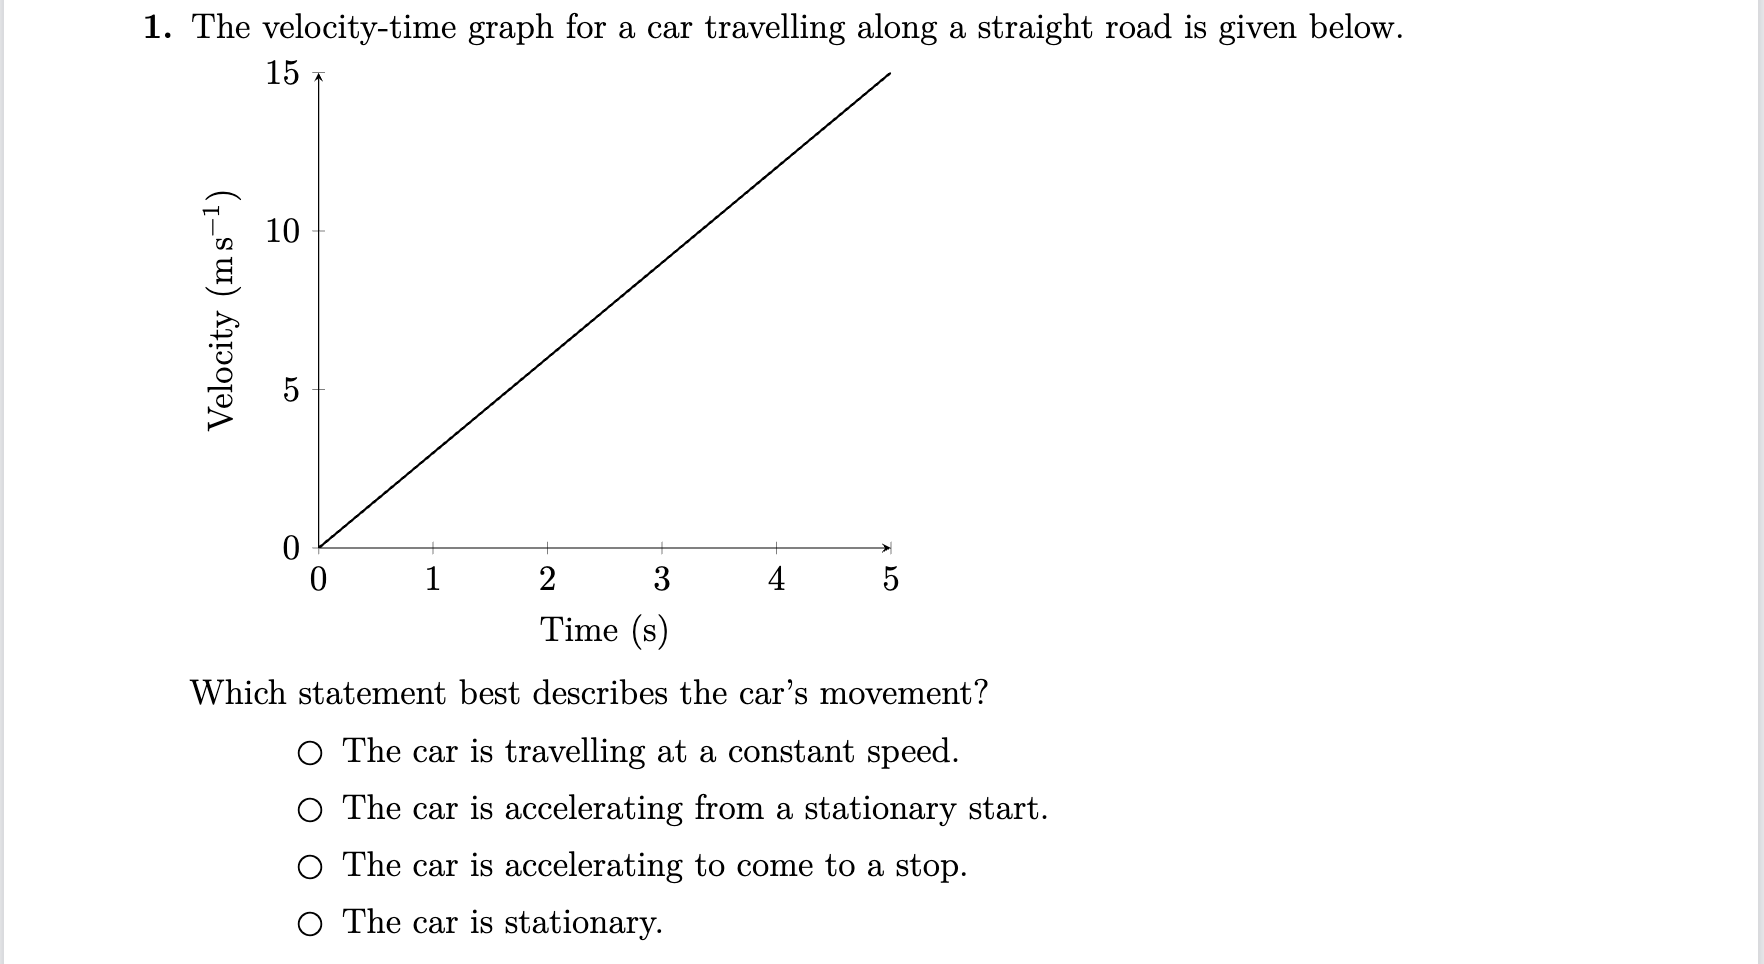
\includegraphics[scale=0.45]{Screenshot multiple choice.png}\\
    \bottomrule
    \end{tabular}
    \caption{Multiple choice question}
    \label{tab:multipleChoice}
\end{table}
If you want to have a separate answer sheet, \LaTeX\ can generate one of those too. There is an example sheet in the appendices on page \pageref{multipleChoiceSheet}.
\subsection{Longer answers}
You probably want to include some questions that are not multiple choice, \LaTeX\ gives you all the normal tools to add subsections with automatic labelling, and these will support their own marks if you want to print them for each part. You can also include other elements in the questions, as we've seen in the earlier sections.
\subsubsection{Including images}
Although \LaTeX\ is powerful, it is probably not worth the effort to write the commands to draw something of photographic quality. Luckily you can include images from external files. I'm going to explain the process for adding an image using Overleaf. If you are using another package, it will have its own instructions.

To add an image to an Overleaf document, you first need to upload it to the Overleaf servers. This is a simple task. There are limits imposed by Overleaf for a free account, but it's 2000 files, each of which can be no larger than \SI{50}{\mega\byte}. Although the total size of a project is unlimited, it is suggested that the whole thing should stay under \SI{500}{\mega\byte}.
\subsection{Prepared working space}
If you want to provide a more structured working environment for students, you can add elements to the exam paper with little difficulty.
\subsubsection{Space for writing}
If you want to leave blank space for a longer answer, you can just use the \textbf{\textbackslash vspace\{50mm\}} command (adjust the 50mm to suit). This will just leave blank space, or use the \textbf{\textbackslash ans} and \textbf{\textbackslash ansl} commands shown on page \pageref{anslCode} which will add the marks for the question.

The \textbf{\textbackslash rule} command will draw a thin horizontal line the width of the page which is suitable for use as an answer line. \textbf{\textbackslash rule} allows you to specify the length of the line (\textbf{\textbackslash textwidth}) for the full width and the thickness of the line.  Generally, you will combine it with a \textbf{\textbackslash vspace\{\}} command to leave enough space between consecutive lines if you need more than one. You can also colour the lines if you prefer.
\begin{table} [H]
\begin{tabular}{m{0.97\textwidth}}
    \toprule
    \LaTeX\ rules (or is that roolz?) \\
    \addlinespace
    \midrule
\vspace{6mm}
\begin{lstinline}!\par\noindent\rule{\textwidth}{0.4pt}!\end{lstinline}
\par\noindent\rule{0.97\textwidth}{0.4pt}\\
\vspace{6mm}
\begin{lstinline}!\par\noindent\rule{0.5\textwidth}{2.0pt}!\end{lstinline}
\par\noindent\rule{0.5\textwidth}{2.0pt}\\
\vspace{6mm}
\begin{lstinline}!\par\noindent{\color{cyan}\rule{\textwidth}{0.4pt}}!\end{lstinline}
\par\noindent {\color{cyan}\rule{0.97\textwidth}{0.4pt}}\\
    \bottomrule
    \caption{Writing lines}
    \label{tab:writingLines}
\end{tabular}
\end{table}
%\def \dotfill#1{\cleaders \hbox to #1{.}\hfill}
%\newcommand{\dotline}[2][.5em]{\leavevmode \hbox to #2{\color{Gray} \dotfill{#1} \hfil}}
%\dotline{}

\subsubsection{Space for graphing}
You can add graph paper grids fairly easily to be used as working area. The \textbf{\textbackslash draw} command lets you adjust the size and spacing and the darkness or lightness of lines. If you need something a bit more complicated, the \texttt{\textbackslash axis} command gives even more choice when you combine it with the grid drawing.
\begin{table} [H]
    \centering
    \begin{tabular}{m{\textwidth}}
    \toprule
    \LaTeX\ \begin{lstinline}!\usepackage{tikzpicture}!\end{lstinline} \\
    \addlinespace
    \midrule
    \begin{lstlisting}
\def\width{12}
\def\height{10}

\begin{tikzpicture}[x=1cm, y=1cm, semitransparent]
\draw[step=2mm, line width=0.1mm, black!30!white] (0,0) grid (\width,\height);
\draw[step=1cm, line width=0.3mm, black!90!white] (0,0) grid (\width,\height);
\end{tikzpicture}
\end{lstlisting}\\
\begin{center}
\def\width{12}
\def\height{10}

\begin{tikzpicture}[x=1cm, y=1cm, semitransparent]
\draw[step=2mm, line width=0.1mm, black!30!white] (0,0) grid (\width,\height);
\draw[step=1cm, line width=0.3mm, black!90!white] (0,0) grid (\width,\height);
\end{tikzpicture}
\end{center}\\
    \bottomrule
    \caption{Plain graph paper}
    \label{tab:plainGraph}
    \end{tabular}
\end{table}

\begin{table} [H]
    \centering
    \begin{tabular}{m{\textwidth}}
    \toprule
    \LaTeX\ \begin{lstinline}!\usepackage{pgfplots}!\end{lstinline} \\
    \addlinespace
    \midrule
    \begin{lstlisting}
\begin{center}
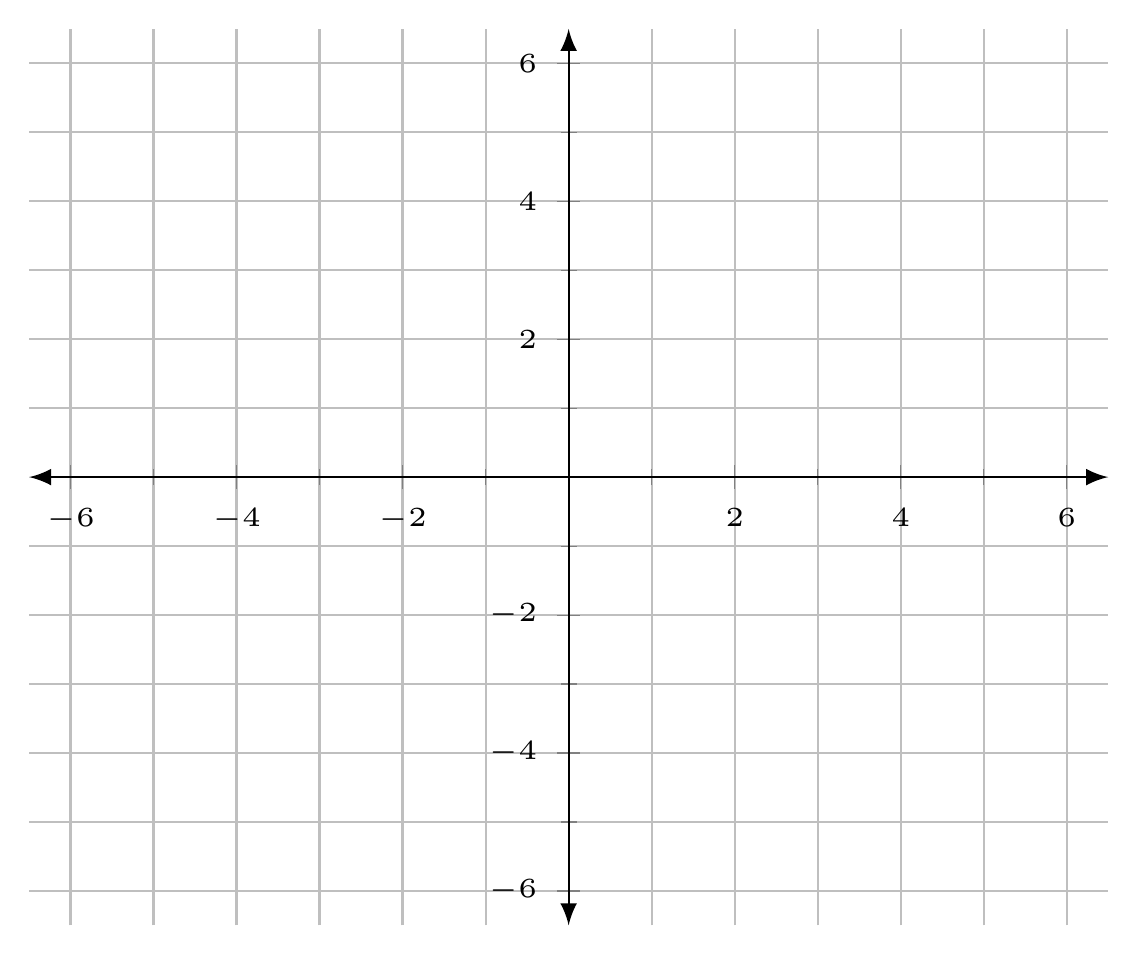
\begin{tikzpicture} [scale=2.0]
\begin{axis}[
    xshift=9cm,
    xmin=-6,xmax=6,
    ymin=-6,ymax=6,
    grid=both,
    axis lines=middle,
    minor tick num=1,
    enlargelimits={abs=0.5},
    axis line style={latex-latex},
    ticklabel style={font=\tiny,fill=none},
    xlabel style={at={(ticklabel* cs:1)},anchor=north west},
    ylabel style={at={(ticklabel* cs:1)},anchor=south west}]
\end{axis}
\end{tikzpicture}
\end{center}
\end{lstlisting}\\
\begin{center}
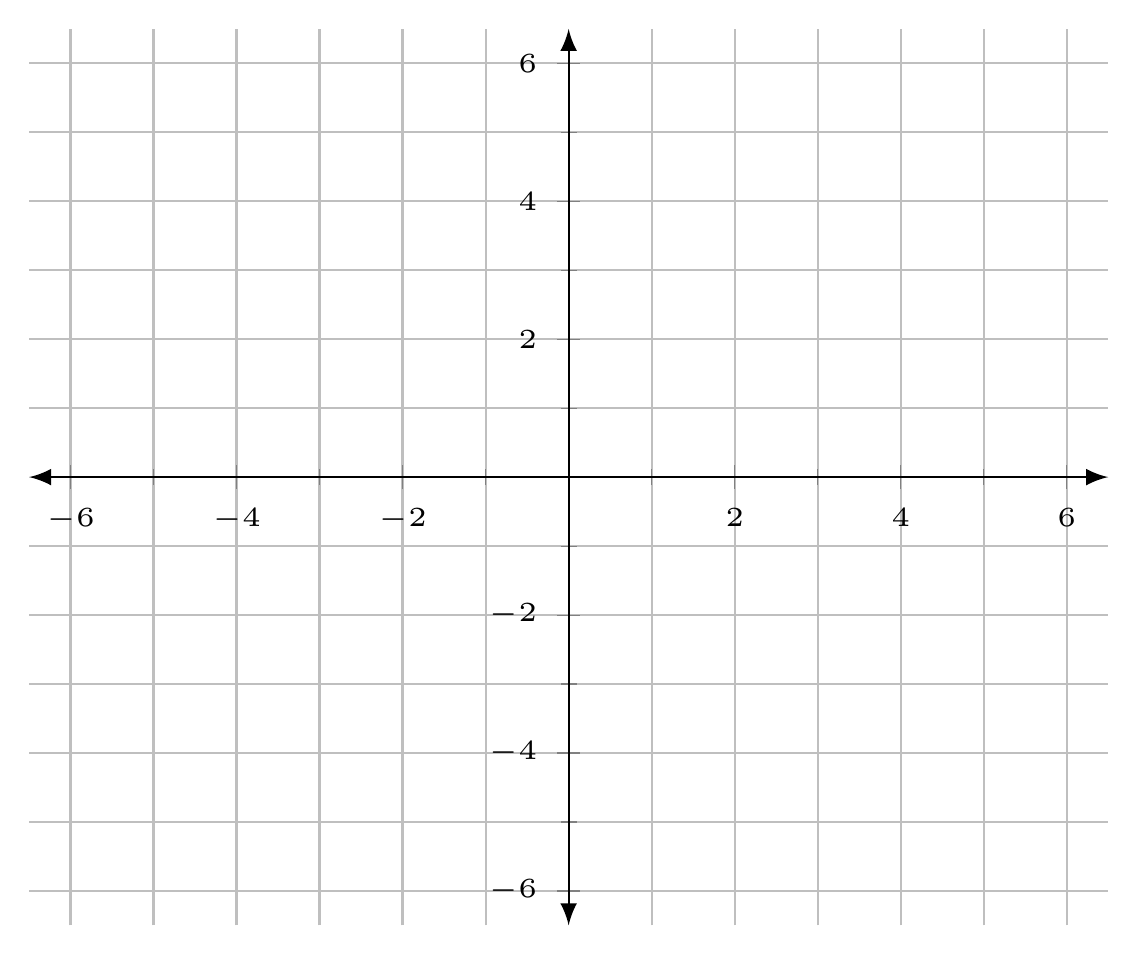
\begin{tikzpicture} [scale=2.0]
\begin{axis}[
    xshift=9cm,
    xmin=-6,xmax=6,
    ymin=-6,ymax=6,
    grid=both,
    axis lines=middle,
    minor tick num=1,
    enlargelimits={abs=0.5},
    axis line style={latex-latex},
    ticklabel style={font=\tiny,fill=none},
    xlabel style={at={(ticklabel* cs:1)},anchor=north west},
    ylabel style={at={(ticklabel* cs:1)},anchor=south west}]
\end{axis}
\end{tikzpicture}
\end{center}\\
    \bottomrule
    \caption{Grid with axes}
    \label{tab:gridAxes}
    \end{tabular}
\end{table}

\section{Accessibility and modifications}
One of the big advantages of using a markup package such as \LaTeX\ is that you can do conditional rendering. In our case, that means we can create one \LaTeX\ document that can produce a number of different PDFs depending upon our settings. Generally, you want a single flag that will make all the changes needed.

A good example might be in the standardised instructions you use on the front page of an assessment task. For some tasks, a calculator will not be allowed; for others, it will be. One approach might be:

\begin{lstlisting}
\newcommand{\nocalculator}{} %comment this line if calculators are allowed
\ifdefined \nocalculator
    \item You may not use a calculator for this task.
\else 
    \item You may use a NESA-approved calculator.
\fi
\end{lstlisting}

There are other ways of doing this, but I find this way to be the most straightforward. In practice, it is a good idea to collect all the flags into one section of the document so that they are easy to find.
\subsection{Conditional modifications}
I have defined a set of four conditional formatting commands for use when modifying a task. The first allows a block of text to be conditionally highlighted to emphasise important words and phrases, the other three allow content to be modified to be included in only the modified document, only the unmodified document, or alternatives depending on the modification state. All of them are controlled by a single line which is commented out for unmodified copies and included for modified ones.
\begin{lstlisting}
\newcommand{\modified}{} % comment this line out for the unmodified version

% Modification formatting
\newcommand{\modHighlight}[1]{\ifdefined \modified \colorbox{orange!30}{#1} \else #1 \fi}
\newcommand{\modOnly}[1]{\ifdefined \modified #1 \fi}
\newcommand{\unmodOnly}[1]{\ifdefined \modified \else #1 \fi}
\newcommand{\modAlternatives}[2]{\ifdefined \modified #2 \else #1 \fi}
\end{lstlisting}

Using the \lstinline|\modHighlight{}| command is as simple as including the text which is to be conditionally highlighted in the braces. If modified is on then the text will be highlighted, otherwise it is left unchanged. I use an orange highlight at 30\% opacity, if you would like something different, just change the \lstinline|{orange!30| to something else in the \lstinline|\newcommand{\modHighlight}| line.\textbf{}

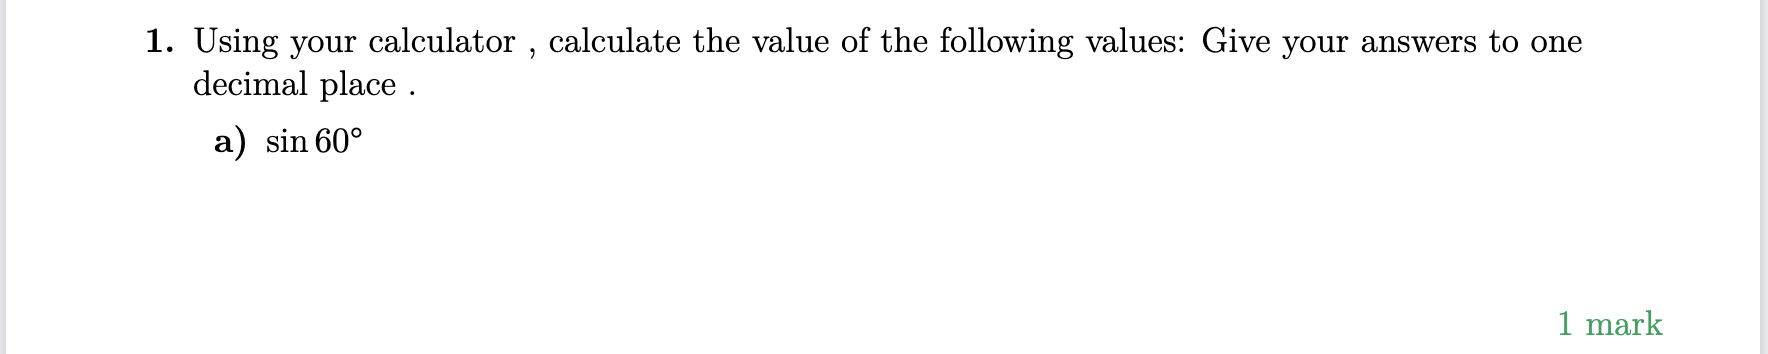
\includegraphics[scale=0.6]{Screenshot NoHighlight.png}
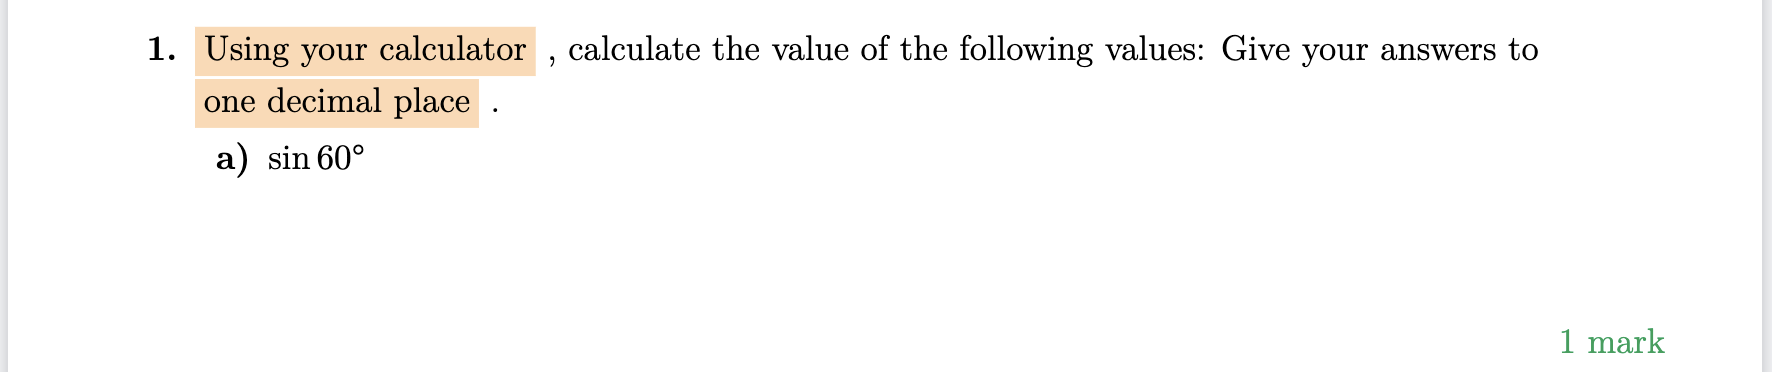
\includegraphics[scale=0.6]{Screenshot Highlight.png}

The \lstinline|\modOnly{}| and \lstinline|\unmodOnly{}| commands both work in the same way. In the braces include the material that should be included in only one version. If adding or omitting material makes a difference to the marking scheme, if you are using the built-in marks with \LaTeX\ the totals will be adjusted automatically and the putput document will be all correct. I think this is one of the best reasons for using \LaTeX\ on anything that has marks associated with it.

The last command \lstinline|\modAlternatives{}{}| takes two sets of content, the first contains the material for the unmodified output, and the second the content for the modified output. Again, if there are different marking implications these will be correctly handled for the different outputs.
\subsection{Support for alternate fonts}
Alternate fonts make your work look nicer, but from an accessibility standpoint, they can make the material more accessible. Because of the support PDF viewers give, we don't need to worry too much about font sizes; PDF readers can scale text and diagrams almost indefinitely. What can make a difference, though, is the font itself.

The Open Dyslexic font has been designed to mitigate some of the common problems associated with dyslexia. It is available for free and may help some students with reading the text portions of material. It can easily be applied to a \LaTeX\ document and is simple enough that it can be offered to students with or without a diagnosis of dyslexia.

Firstly you need to add the Open Dyslexic font to your system, which is done in the normal way for your computer. Then adding support for the font is simple. Two commands need to be added to the preamble section of your document.
\begin{lstlisting}
\usepackage{fontspec}
\setmainfont{OpenDyslexic}
\end{lstlisting}

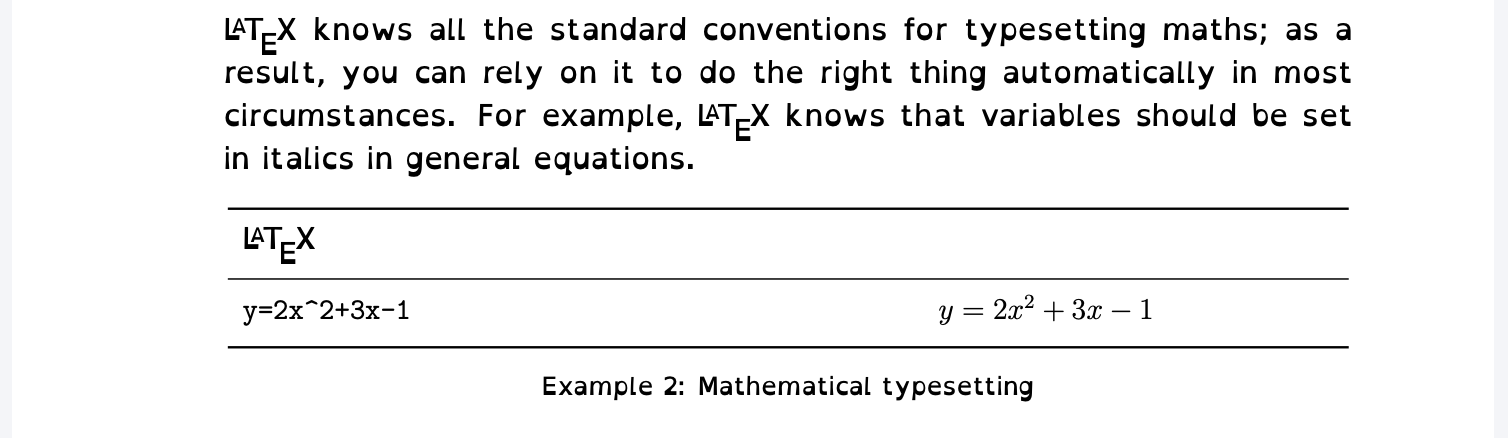
\includegraphics[scale=0.6]{Screenshot opendyslexic.png}

Using the Open Dyslexic font will only change the text portions of the document; it will not change the material set using the maths functions or other special formatting, such as code listings.
\subsection{Support for low-vision users}
As the output from a \LaTeX\ file is a PDF document, a low-vision user can take advantage of the fact that because a PDF is a vector format, it is effectively infinitely scalable, making it very simple to enlarge the document on screen as much as needed. Similarly, a PDB document can be reversed to show white text on a black background. Tools such as Adobe Acrobat can allow even more flexibility with colour changes for text and background.

There are two packages that you need to add to your document's preamble to have it make PDFs for users for whom no visual representation is suitable. The packages are \textbf{accessibility} and \textbf{axessibility}. The first allows you to add alt text to the images in your document. This will be turned into tags in the final PDF which will be accessed by screen reader technologies. You simply add the \lstinline|\alt{description}| tag inside the \lstinline|\figure| tag and the description will go into PDF correctly.

The \textbf{axessibility} package allows for mathematical equations to be read out correctly by a screen reader. To use it, equations have to be surrounded by \lstinline|\begin{equation}| and \lstinline|\end{equation}|, so it's a bit more work. Once you have an accessible file, there are online services that can convert it into an audio file for users who may not be able to use a screen reader.
\subsubsection{Braille}
Because it's a PDF, a \LaTeX document can be converted to Braille via an online service such as RoboBraille.org. 
\section{How do I…}
This section is made up of all the things that I needed to do to get this paper typeset using \LaTeX\ which aren't covered in other parts of the paper. It's definitely not everything that you'll need to know, but luckily \LaTeX\ has been around for a long time, and as it's open source, there are thousands of pages of information available on the Internet.
\subsection{How do I change the default text size of my document?}
The only sizes available in standard \LaTeX \space are 10pt, 11pt and 12pt; if those are the only sizes you need, then right at the top of your document, add the new default font size to the \texttt{$\backslash$documentclass} element like this:

\lstinline|\documentclass[12pt]{article}|

If you set it to any other value than 10, 11 or 12, it will just default to 10pt.

It is quite likely that you will want a font size that is outside the range available. You can do this by making a small change to the \texttt{$\backslash$documentclass} element, simply change \texttt{article} to \texttt{extarticle}.

\lstinline|\documentclass[14pt]{extarticle}|

Note that when you change the base text size of your document, all the other standard elements like titles and subtitles will also change their default sizes to match.
\subsection{How do I change the document's font?}
If you need to change the font in just a small area, need to set the font up in the preamble.

\begin{lstlisting}
\usepackage[T1]{fontenc}
\usepackage{tgheros}
\end{lstlisting}

The \lstinline|tgheros| is the name of the font package, which contains the set of fonts. To use the font within the document you use the \lstinline|\fontfamily{}| command with \lstinline|\selectfont{}|.
\begin{lstlisting}
 {\fontfamily{qhv}\selectfont
This text uses a different font typeface}   
\end{lstlisting}
Which produces:
{\fontfamily{qhv}\selectfont
This text uses a different font typeface}\\
Except that as you can see, it didn't. That's because using this command in a document with a lot of mathematical typesetting causes the maths symbols to be replaced by other characters.

If you want to change it for the entire document, you need to add some settings to the document's preamble.

\begin{center}
\begin{lstlisting}   
\usepackage{fontspec}
\setmainfont{Helvetica}
\end{lstlisting}
\end{center}

Just set the name of the font to one of the installed fonts on your computer. For this to work properly, you need to be using either the LuaLaTeX or XeLaTeX engines to make your document.

\begin{lstlisting}
\fontencoding{T1}
\fontfamily{garamond}
\fontseries{m}
\fontshape{it}
\fontsize{12}{15}
\selectfont
\end{lstlisting}

These commands will change the font to Garamond, 
\subsection{How do I change the colour or style of my text?}
To get a good range of colours in \LaTeX\, include \lstinline|\usepackage{xcolor}| in the preamble. To change the colour of text, include the text in braces with the \lstinline|\color{}{}| command. For example \lstinline|\textcolor{teal}{This is coloured text.}| will render as \textcolor{teal}{This is coloured text.} There are other packages that give access to even more colours; for instance, \lstinline|\usepackage[x11names]{xcolor}| adds another 68 CMYK colours.

To make a section of text \textbf{bold face}, surround it with \lstinline|\textbf{ }|.

If you want \textit{italicised text}, use \lstinline|\textit{ }|.

\underline{Underlining} is done with \lstinline|\underline{ }|.

\subsection{How do I put a block of code into my text?}
There are two ways of adding code into text, depending on whether you need to render a lot or just a little. The problem we need to overcome is how \LaTeX\ knows that we want to print the code rather than render it. These techniques also work if you want to show code in computer languages that use special characters which are the same as the ones \LaTeX\ uses.

For a small amount of text, the easiest thing is to start with \lstinline{\lstinline|} followed by the text and then \lstinline{|} to finish. That \lstinline{|} character is the vertical bar found under the delete key; it's called the pipe character. If you need to have a pipe character in the text, then you can use \lstinline|\lstinline{ }| instead. If you need both pipes and braces, use \lstinline{\lstinline| |}, put the braces in your text normally and use \lstinline{$|$} for the pipes.

If you need a multiline block of code, use \lstinline|\begin{lstlisting}| and \lstinline|\end{lstlisting}| and put the code in between. You can adjust the indenting of the rendered lines in the text by adjusting them within the block. If you are using Overleaf, you will notice that it colours the code text differently to make it easier to identify when you are looking at your work.

\subsection{How do I get a space after using a \LaTeX\ command?}
By default, when you use a \LaTeX\ command that produces text in amongst other text, it will not leave a space after the command. This might seem strange, but it turns out to be fairly useful. Luckily it is very simple to get \LaTeX\ to leave a space; just add an extra \textbf{\textbackslash} to the end of the \LaTeX\ command.
\subsection{How do I include a \textbackslash\ in my text?}
Because the backslash character is used so extensively in \LaTeX\ it can be difficult to get it to print normally. There are all sorts of workarounds, but the simplest is to just use the command \lstinline|\textbackslash| in your text.
\subsection{How do I add a header or footer?}
Different types of \LaTeX\ documents handle headers and footers in slightly different ways. If you are using the exam type, you can use them like this:
\begin{lstlisting}
\pagestyle{headandfoot} 
\firstpageheader{}{}{\vspace{1em} Name: \dotline[2pt]{80mm}}
\runningheader{\textcolor{Gray}\ClassName}{\textcolor{Gray}\ExamName}{\textcolor{Gray}{Initials: \dotline[2pt]{2cm}}}
\runningfooter{\modOnly{\textcolor{Gray}{Modified}}}{\textcolor{Gray}{Page \thepage\ of \pageref{lastpage}}}{\textcolor{Gray}{\textbf{/ \pointsonpage{\thepage}}}}
\end{lstlisting}
In this section of an exam paper, we start by letting \LaTeX\ know that we want to include a header and footer. The following lines define each of the headers and footers. Here we have defined a header for the first page, a header for all the subsequent pages, and a footer for all the pages after the first. There are a few different types of headers and footers available, including odd and even pages if you are using a document type with that setting.

\subsection{How do I get better paragraph spacing?}
The easiest way to get nice paragraph spacing is to include the \texttt{parskip} package. Just add the line

\lstinline|\usepackage{parskip}|

in the header section of your document. This will give you paragraphs separated by an empty line and no indenting. It's the style used in this document. Of course, there are lots of other options available as well.
\subsection{Why are my quote marks wrong?}
The problem comes from the fact that you are using the standard double quote character on your keyboard to include quotes. Instead, you need to use \space $\grave{}$ \space $\grave{}$ (the key next to the 1, twice) for the leading quotes and ' ' (the key next to the return key, twice) for the trailing quotes. No, I don't know why they did it that way.
\subsection{How do I add a cross-reference or a page number reference?}\label{cross-reference-location}
Adding references is a two-part process; the first part is to label the location that you are going to want to cross-reference. This is done by adding a \lstinline|\label{label-name-here}| command to the item being referenced. The name you use for the label needs to be unique throughout the document.

The second part is to make the reference; the \lstinline|\ref{reference-name}| command is used. That command is being used to create the entry that this section is numbered $\ref{cross-reference-location}$, and it is on page \pageref{cross-reference-location}.

The page number comes from using the \lstinline|\pageref{label-name-here}|
command. Of course, you can refer to a reference as many times as you like.
\subsection{Extra features}
There are lots of little things that have been added to \LaTeX\ over the years. Far too many to mention here, so here are some that I have found useful.

The table of contents and list of examples that are included at the start of this document are both generated automatically by \LaTeX. In each case, they take only one command to create and properly format the sections; they even do useful things like leaving out their own entries. The table of contents builds itself from the headings you put in the document and the list of examples from the captions you put on figures. It even lets you call them examples rather than figures.

You can generate cross-references and page references just by adding a label to the document.

\LaTeX\ integrates with pieces of bibliographic software so references can be added to work automatically and in a choice of formats. The paid version also integrates with Dropbox and GitHub.
\section{Appendices}
\subsection{Graph paper and writing paper}
\subsection{Multiple choice answer sheet}
\label{multipleChoiceSheet}
This code will generate a block of 4 letter answer lines for multiple choice questions. Change the number in the \lstinline|\def\qCount{20}| command near the end.
\label{LastPage}
\end{document}